%% abtex2-modelo-trabalho-academico.tex, v-1.9.2 laurocesar
%% Copyright 2012-2014 by abnTeX2 group at http://abntex2.googlecode.com/
%%
%% This work may be distributed and/or modified under the
%% conditions of the LaTeX Project Public License, either version 1.3
%% of this license or (at your option) any later version.
%% The latest version of this license is in
%%   http://www.latex-project.org/lppl.txt
%% and version 1.3 or later is part of all distributions of LaTeX
%% version 2005/12/01 or later.
%%
%% This work has the LPPL maintenance status `maintained'.
%%
%% The Current Maintainer of this work is the abnTeX2 team, led
%% by Lauro César Araujo. Further information are available on
%% http://abntex2.googlecode.com/
%%
%% This work consists of the files abntex2-modelo-trabalho-academico.tex,
%% abntex2-modelo-include-comandos and abntex2-modelo-references.bib
%%

% ------------------------------------------------------------------------
% ------------------------------------------------------------------------
% abnTeX2: Modelo de Trabalho Academico (tese de doutorado, dissertacao de
% mestrado e trabalhos monograficos em geral) em conformidade com
% ABNT NBR 14724:2011: Informacao e documentacao - Trabalhos academicos -
% Apresentacao
% ------------------------------------------------------------------------
% ------------------------------------------------------------------------

\documentclass[
	% -- opções da classe memoir --
	12pt,				% tamanho da fonte
	openright,			% capítulos começam em pág ímpar (insere página vazia caso preciso)
	twoside,			% para impressão em verso e anverso. Oposto a oneside
	a4paper,			% tamanho do papel.
	% -- opções da classe abntex2 --
	%chapter=TITLE,		% títulos de capítulos convertidos em letras maiúsculas
	%section=TITLE,		% títulos de seções convertidos em letras maiúsculas
	%subsection=TITLE,	% títulos de subseções convertidos em letras maiúsculas
	%subsubsection=TITLE,% títulos de subsubseções convertidos em letras maiúsculas
	% -- opções do pacote babel --
	english,			% idioma adicional para hifenização
	french,				% idioma adicional para hifenização
	spanish,			% idioma adicional para hifenização
	brazil				% o último idioma é o principal do documento
	]{abntex2}

% ---
% Pacotes básicos
% ---
\usepackage{lmodern}			% Usa a fonte Latin Modern
\usepackage[T1]{fontenc}		% Selecao de codigos de fonte.
\usepackage[utf8]{inputenc}		% Codificacao do documento (conversão automática dos acentos)
\usepackage{lastpage}			% Usado pela Ficha catalográfica
\usepackage{indentfirst}		% Indenta o primeiro parágrafo de cada seção.
\usepackage{color}				% Controle das cores
\usepackage{graphicx}			% Inclusão de gráficos
\usepackage{microtype} 			% para melhorias de justificação
\usepackage[final]{pdfpages}
\usepackage{url}
\usepackage{float}
\usepackage{amsmath}
\usepackage{cleveref}
\usepackage{pgfplots}
\pgfplotsset{compat=1.17}
\usepackage{amsfonts}
\usepackage{amsmath}
\usepackage{tikz}
\usetikzlibrary{matrix, positioning}
\usepackage{tabularx}
\usepackage{mathtools}
\DeclareMathOperator{\logsumexp}{logsumexp}
\pgfmathdeclarefunction{sumexp}{3}{%
  \begingroup%
  \pgfkeys{/pgf/fpu}% "/pgf/fpu/output format=fixed" removed
  \pgfmathsetmacro{\myx}{#1}%
  \pgfmathtruncatemacro{\myxmin}{#2}%
  \pgfmathtruncatemacro{\myxmax}{#3}%
  \pgfmathsetmacro{\mysum}{0}%
  \pgfplotsforeachungrouped\XX in {\myxmin,...,\myxmax}%
    {\pgfmathsetmacro{\mysum}{\mysum+exp(\XX)}}%
  \pgfmathparse{\mysum+exp(#1)}%
  \pgfmathfloattofixed\pgfmathresult%  added
  \pgfmathsmuggle\pgfmathresult\endgroup%
}


\crefname{figure}{Figura}{Figuras}
\crefname{equation}{Equação}{Equações}
% ---

% ---
% Pacotes adicionais, usados apenas no âmbito do Modelo Canônico do abnteX2
% ---
\usepackage{lipsum}				% para geração de dummy text
% ---

% ---
% Pacotes de citações
% ---
\usepackage[brazilian,hyperpageref]{backref}	 % Paginas com as citações na bibl
\usepackage[alf]{abntex2cite}	% Citações padrão ABNT

% ---
% CONFIGURAÇÕES DE PACOTES
% ---

% ---
% Configurações do pacote backref
% Usado sem a opção hyperpageref de backref
\renewcommand{\backrefpagesname}{Citado na(s) página(s):~}
% Texto padrão antes do número das páginas
\renewcommand{\backref}{}
% Define os textos da citação
\renewcommand*{\backrefalt}[4]{
	\ifcase #1 %
		Nenhuma citação no texto.%
	\or
		Citado na página #2.%
	\else
		Citado #1 vezes nas páginas #2.%
	\fi}%
% ---

% ---
% Informações de dados para CAPA e FOLHA DE ROSTO
% ---
\titulo{{Geração Procedural de Mapas para Jogos através da Segmentação de Imagens por Rede Neural Convolucional}}
\autor{Lucas da Silva dos Santos\\Matheus Zanivan Andrade\\ Rafael Nascimento Lourenço}
\local{São Paulo - Brasil}
\data{2023}
\orientador{Thyago Conchado Quintas}
% \coorientador{Equipe \abnTeX}
\instituicao{%
  Centro Universitário Senac - Santo Amaro
  \par
  Bacharelado em Ciência da Computação
}
\tipotrabalho{Trabalho de Conclusão de Curso (TCC)}
% O preambulo deve conter o tipo do trabalho, o objetivo,
% o nome da instituição e a área de concentração
\preambulo{Monografia apresentada na disciplina Trabalho de Conclusão de Curso, como parte dos requisitos para obtenção do título de Bacharel em Ciência da Computação.}
% ---


% ---
% Configurações de aparência do PDF final

% alterando o aspecto da cor azul
\definecolor{blue}{RGB}{41,5,195}

% informações do PDF
\makeatletter
\hypersetup{
     	%pagebackref=true,
		pdftitle={\@title},
		pdfauthor={\@author},
    	pdfsubject={\imprimirpreambulo},
	    pdfcreator={LaTeX with abnTeX2},
		pdfkeywords={abnt}{latex}{abntex}{abntex2}{trabalho acadêmico},
		colorlinks=true,       		% false: boxed links; true: colored links
    	linkcolor=blue,          	% color of internal links
    	citecolor=blue,        		% color of links to bibliography
    	filecolor=magenta,      		% color of file links
		urlcolor=blue,
		bookmarksdepth=4
}
\makeatother
% ---

% ---
% Espaçamentos entre linhas e parágrafos
% ---

% O tamanho do parágrafo é dado por:
\setlength{\parindent}{1.3cm}

% Controle do espaçamento entre um parágrafo e outro:
\setlength{\parskip}{0.2cm}  % tente também \onelineskip

% ---
% compila o indice
% ---
\makeindex
% ---

% ----
% Início do documento
% ----
\begin{document}

% Retira espaço extra obsoleto entre as frases.
\frenchspacing

% ----------------------------------------------------------
% ELEMENTOS PRÉ-TEXTUAIS
% ----------------------------------------------------------
% \pretextual

% ---
% Capa
% ---
\imprimircapa
% ---

% ---
% Folha de rosto
% (o * indica que haverá a ficha bibliográfica)
% ---
\imprimirfolhaderosto*
% ---

% ---
% Inserir a ficha bibliografica
% ---
% Isto é um exemplo de Ficha Catalográfica, ou ``Dados internacionais de
% catalogação-na-publicação''. Você pode utilizar este modelo como referência.
% Porém, provavelmente a biblioteca da sua universidade lhe fornecerá um PDF
% com a ficha catalográfica definitiva após a defesa do trabalho. Quando estiver
% com o documento, salve-o como PDF no diretório do seu projeto e substitua todo
% o conteúdo de implementação deste arquivo pelo comando abaixo:
%
% \begin{fichacatalografica}
%     \includepdf{ficha.pdf}
% \end{fichacatalografica}
% ---

% ---
% Inserir errata
% ---
% \begin{errata}
% Elemento opcional da \space\citeonline[4.2.1.2]{NBR14724:2011}. Exemplo:

% \vspace{\onelineskip}

% FERRIGNO, C. R. A. \textbf{Tratamento de neoplasias ósseas apendiculares com
% reimplantação de enxerto ósseo autólogo autoclavado associado ao plasma
% rico em plaquetas}: estudo crítico na cirurgia de preservação de membro em
% cães. 2011. 128 f. Tese (Livre-Docência) - Faculdade de Medicina Veterinária e
% Zootecnia, Universidade de São Paulo, São Paulo, 2011.

% \begin{table}[htb]
% \center
% \footnotesize
% \begin{tabular}{|p{1.4cm}|p{1cm}|p{3cm}|p{3cm}|}
%   \hline
%    \textbf{Folha} & \textbf{Linha}  & \textbf{Onde se lê}  & \textbf{Leia-se}  \\
%     \hline
%     1 & 10 & auto-conclavo & autoconclavo\\
%    \hline
% \end{tabular}
% \end{table}

% \end{errata}
% ---

% ---
% Inserir folha de aprovação
% ---

% Isto é um exemplo de Folha de aprovação, elemento obrigatório da NBR
% 14724/2011 (seção 4.2.1.3). Você pode utilizar este modelo até a aprovação
% do trabalho. Após isso, substitua todo o conteúdo deste arquivo por uma
% imagem da página assinada pela banca com o comando abaixo:
%
% \includepdf{folhadeaprovacao_final.pdf}
%
\begin{folhadeaprovacao}

  \begin{center}
    {\ABNTEXchapterfont\large\imprimirautor}

    \vspace*{\fill}\vspace*{\fill}
    \begin{center}
      \ABNTEXchapterfont\bfseries\Large\imprimirtitulo
    \end{center}
    \vspace*{\fill}

    \hspace{.45\textwidth}
    \begin{minipage}{.5\textwidth}
        \imprimirpreambulo
    \end{minipage}%
    \vspace*{\fill}
   \end{center}

%    Trabalho aprovado. \imprimirlocal, 24 de novembro de 2012:

   \assinatura{\textbf{\imprimirorientador} \\ Orientador}
   \assinatura{\textbf{Professor} \\ Convidado 1}
   \assinatura{\textbf{Professor} \\ Convidado 2}
   %\assinatura{\textbf{Professor} \\ Convidado 3}
   %\assinatura{\textbf{Professor} \\ Convidado 4}

   \begin{center}
    \vspace*{0.5cm}
    {\large\imprimirlocal}
    \par
    {\large\imprimirdata}
    \vspace*{1cm}
  \end{center}

\end{folhadeaprovacao}
% ---

% ---
% Dedicatória
% ---
\begin{dedicatoria}
   \vspace*{\fill}
   \centering
   \noindent
   \textit{ Este trabalho é dedicado às crianças adultas que,\\
   quando pequenas, sonharam em se tornar cientistas.} \vspace*{\fill}
\end{dedicatoria}
% ---

% ---
% Agradecimentos
% ---
% \begin{agradecimentos}
% Os agradecimentos principais são direcionados à Gerald Weber, Miguel Frasson,
% Leslie H. Watter, Bruno Parente Lima, Flávio de Vasconcellos Corrêa, Otavio Real
% Salvador, Renato Machnievscz\footnote{Os nomes dos integrantes do primeiro
% projeto abn\TeX\ foram extraídos de
% \url{http://codigolivre.org.br/projects/abntex/}} e todos aqueles que
% contribuíram para que a produção de trabalhos acadêmicos conforme
% as normas ABNT com \LaTeX\ fosse possível.

% Agradecimentos especiais são direcionados ao Centro de Pesquisa em Arquitetura
% da Informação\footnote{\url{http://www.cpai.unb.br/}} da Universidade de
% Brasília (CPAI), ao grupo de usuários
% \emph{latex-br}\footnote{\url{http://groups.google.com/group/latex-br}} e aos
% novos voluntários do grupo
% \emph{\abnTeX}\footnote{\url{http://groups.google.com/group/abntex2} e
% \url{http://abntex2.googlecode.com/}}~que contribuíram e que ainda
% contribuirão para a evolução do \abnTeX.

% \end{agradecimentos}
% ---

% ---
% Epígrafe
% ---
% \begin{epigrafe}
%     \vspace*{\fill}
% 	\begin{flushright}
% 		\textit{``Não vos amoldeis às estruturas deste mundo, \\
% 		mas transformai-vos pela renovação da mente, \\
% 		a fim de distinguir qual é a vontade de Deus: \\
% 		o que é bom, o que Lhe é agradável, o que é perfeito.\\
% 		(Bíblia Sagrada, Romanos 12, 2)}
% 	\end{flushright}
% \end{epigrafe}
% ---

% ---
% RESUMOS
% ---

% resumo em português
\setlength{\absparsep}{18pt} % ajusta o espaçamento dos parágrafos do resumo
\begin{resumo}
  Esta monografia descreve o desenvolvimento de uma ferramenta para jogos que oferece uma nova funcionalidade. A ferramenta começa com a seleção de uma foto, que é processada por um modelo de rede neural convolucional especializado em segmentação panóptica. Isso permite a segmentação da imagem, incluindo a separação de objetos da mesma classe, como pessoas e carros. Após o modelo gerar a imagem de saída, será possível selecionar um contorno detectado e, a partir disso, gerar um mapa de forma procedural, combinado com o diagrama de Voronoi para criar os biomas do mapa.

 \textbf{Palavras-chaves}: segmentação panóptica, geração procedural, diagrama de Voronoi, mapas, jogos.
\end{resumo}

% resumo em inglês
\begin{resumo}[Abstract]
 \begin{otherlanguage*}{english}
  This monograph describes the development of a tool for games that offers new functionality. The tool starts with the selection of a photo, which is processed by a convolutional neural network model specialized in panoptic segmentation. This allows for the segmentation of the image, including the separation of objects of the same class, such as people and cars. After the model generates the output image, it will be possible to select a detected outline and, from that, generate a procedural shape map, combined with the Voronoi diagram to create the biomes of the map.

   \textbf{Key-words}: panoptic segmentation, procedural generation, Voronoi diagram, maps, games.
 \end{otherlanguage*}
\end{resumo}
% ---

% ---
% inserir lista de ilustrações
% ---
\pdfbookmark[0]{\listfigurename}{lof}
\listoffigures*
\cleardoublepage
% ---

% ---
% inserir lista de tabelas
% ---
\pdfbookmark[0]{\listtablename}{lot}
\listoftables*
\cleardoublepage
% ---

% ---
% inserir lista de abreviaturas e siglas
% ---
\begin{siglas}
  \item[IA] Inteligência Artificial
  \item[RGB] Red, Green and Blue ou Vermelho, Verde e azul
  \item[RNC] Rede Neural Convolucional
  \item[CNN] Convolutional Neural Network
  \item[RTC] Rede Totalmente Convolucional
  \item[RoI] Region of Interest ou Região de interesse
  \item[IoU] Intersection over Union ou União sobre intersecção
  \item[RPC] Pirâmide de Características
  \item[ECLE] Extrator de Características em Larga Escala
  \item[RPR] Rede de Proposta de Região
\end{siglas}
% ---

% ---
% inserir lista de símbolos
% ---
% \begin{simbolos}
%   \item[IA] inteligência Artificial
% \end{simbolos}
% ---

% ---
% inserir o sumario
% ---
\pdfbookmark[0]{\contentsname}{toc}
\tableofcontents*
\cleardoublepage
% ---



% ----------------------------------------------------------
% ELEMENTOS TEXTUAIS
% ----------------------------------------------------------
\textual

% ----------------------------------------------------------
% Introdução (exemplo de capítulo sem numeração, mas presente no Sumário)
% ----------------------------------------------------------
\chapter{Introdução}
% ----------------------------------------------------------

% introduzindo a jogos, por que é um mercado que está tao em alta
A indústria de jogos digitais cresce cada vez mais. De acordo com \space\citeonline{quanto_games_vao_movimentar}, essa indústria tende a ultrapassar em 2023, os US\$ 200 bilhões (aproximadamente, R\$ 1 trilhão). Novos jogos são produzidos e publicados diariamente, e somente na plataforma digital Steam, foram 10.963 novos títulos em 2022\space
\cite{numero_de_jogos_publicados_na_steam}.

% aqui a gente aproveita que falou de jogos para introduzir MAPAS que é o 'tema' do tcc
No cenário de jogos, os mapas desempenham um papel fundamental, fornecendo orientação aos jogadores e criando a sensação de escala em uma área. Por exemplo o jogo de aventura pirata chamado Sea of Thieves, os mapas revelam locais de interesse, como tesouros escondidos, missões e áreas perigosas, além de ajudar os jogadores a planejar suas estratégias, explorar o mundo virtual e tomar decisões com base em informações espaciais. Portanto os mapas enriquecem a experiência geral do jogo, mas cria-los pode ser um desafio, especialmente levando em consideração o orçamento disponível. Pois demandaria muitos recursos criar vários mapas diferentes com intuito de entretenimento do jogador. Em jogos como Minecraft, um elemento importante é a forma procedural no qual se cria os mundos, com ilhas contendo biomas, cavernas, vilas, dentre outros recursos. Com essa diversidade de características pode-se evitar o tédio de sempre jogar no mesmo mapa \space\cite{video-game-maps, lecafedugeek}.

% \begin{figure}[ht]
% 	\caption{Mapa de tesouro do jogo Sea of Thieves}
% 	\centering % para centralizarmos a figura
% 	\includegraphics[width=10cm]{figures/Treasure_Map.jpg} % leia abaixo
% 	\legend{Fonte: \space\citeonline{seaofthieves}}
% 	\label{fig:treasureMap}
% \end{figure}

% aqui a gente faz um adendo e a demanda de jogos tende a crescer, então da a entender que voce tem que produzir cada vez mais
% e tambem fala o quanto custa para produzir um jogo
% Ademais, o mercado de jogos no Brasil teve um aumento de 2,5\% em 2022, como apontado por uma pesquisa sobre o crescimento da demanda \space \space\cite{pesquisa_games_brasil}. O custo de produção de jogos varia bastante, dependendo do tamanho e da complexidade do projeto, \emph{e.g.}, a empresa Rockstar Games revelou que o jogo \textit{Grand Theft Auto V} custou cerca de 265 milhões de dólares para ser desenvolvido e comercializado \space \space\cite{gta_quanto_custou}.

%solucao para o problema
% Apesar do rápido crescimento da indústria, existe uma carência de ferramentas que possam auxiliar os designers e artistas durante o processo de produção de jogos, o que acaba tornando-o demorado e, consequentemente, mais caro.  Segundo o livro "Procedural Content Generation in Games" \space\cite{procedural_centent_book}, uma abordagem eficiente para reduzir os custos de produção de um jogo é utilizar a geração procedural de conteúdo. Essa técnica permite maximizar o desenvolvimento de um jogo, envolvendo o uso de um software de computador capaz de criar conteúdo de jogos automaticamente. Esse software possibilita a geração automatizada de mapas, otimizando o processo de desenvolvimento.


% No entanto, a criação de mapas usando esse método ainda encontram dificuldades, sendo elas, variedade e autenticidade \space\cite{geracao_procedural_jogos_2d}.
% aqui adicionar uma explicação do porque é um desafio a geração procedeural de conteudo

% introduz a relação de ia para personalização dentro de métodos procedurais em jogos
De acordo com \space\citeonline{jogo_procedural} é muito comum usar técnicas procedurais combinado com inteligência artificial para melhorar ou personalizar a experiência do jogador. Por exemplo, o jogo RimWorld é um simulador de colônia que gera um planeta de forma procedural e utiliza uma IA para narrar a história, abrangendo psicologia, ecologia, combate e diplomacia, dentre outros. Logo, essa combinação entre IA e a geração procedural cria uma jogabilidade única ao jogador.

% A aplicação da IA em jogos não se limita apenas à jogabilidade. Ela também é usada em áreas como animação de personagens, reconhecimento de fala e expressões faciais, tradução automática de idiomas nos diálogos do jogo e muito mais. A IA está impulsionando a inovação e a evolução dos jogos, proporcionando experiências cada vez mais envolventes e cativantes para os jogadores \space\cite{exameNvidia, omniverseace}.

% introduz o ramo de segmentação geral que será explicado mais para frente
Em IA, um ramo que está em ascensão é o de segmentação de imagem com redes neurais convolucionais, onde é possível classificar os pixeis de uma imagem e criar máscaras  para destacar cada objeto\footnote{Todas classes que são contáveis como pessoas, carros, etc.} detectado. As suas aplicações são diversas, como por exemplo carros ou drones autônomos, sistemas de vigilância, sistemas militares inteligentes, entre outros.
Na aplicação de carros autônomos é necessário identificar humanos para tomar decisões de freio, em sistemas de vigilância é necesário identificar para alertar e automatizar o processo de segurança, em drones autonomôs para checar a pessoa correspondente a entrega. Portanto, nessas aplicações observa-se que é preciso ter um foco em identificar e segmentar seres humanos para a tomada de decisões \space\cite{dp_semantic_segmantation}.

% Nessas aplicações é possível observar que é preciso ter um foco em identificar e segmentar seres humanos, por exemplo, em carros autônomos é primordial essa tarefa para o carro tomar a decisão de frear quando estiver muito perto de bater.

Logo, se torna um tópico relevante dentro de visão computacional, no qual pode ter diversas aplicações no mundo real \space\cite{kirillov2019panoptic, dp_semantic_segmantation}.

Por conseguinte, a combinação entre inteligência artificial e geração procedural de mapas pode abrir novas possibilidades de personalização nos jogos. Imagine um jogo em que, a partir da segmentação de imagens por meio de redes neurais convolucionais, os jogadores possam criar mapas únicos e personalizados para suas aventuras. Com uma foto, o modelo treinado segmentaria a imagem para selecionar um contorno reconhecido, e a partir dele se criar um mapa de maneira procedural contendo biomas no mesmo formato escolhido.

No contexto da geração procedural de mapas, explorar a relação entre IA e personalização de jogos contribuirá para o avanço dessas áreas de pesquisa, proporcionando aos jogadores experiências mais ricas e variadas.

% Adicionar uma parte explicando a parte de visão computacional e porque o tema da nossa Ia é identificação de pessoas

% Dito isso, nosso projeto tem a ideia de fornecer recursos baseados em matemática aplicada dentro de ciência da computação que proporcione uma funcionalidade de escolher o contorno do mapa no qual irá jogar através de imagens. Abordaremos a arquitetura de redes neurais convolucionais, que é muito utilizada para trabalhar com imagens. Mais especificamente, abordaremos uma arquitetura derivada da arquitetura mencionada anteriormente, específica para segmentação de imagens, o que possibilita classificar contornos em imagens.

\section{Objetivos}

O objetivo principal deste trabalho é desenvolver uma ferramenta que ofereça uma alternativa para a geração procedural de mapas de ilhas, utilizando o diagrama de Voronoi para a criar biomas. Além disso, pretende-se combinar segmentação com redes neurais convolucionais para permitir a personalização desses mapas. Essa ferramenta terá a capacidade de reconhecer os contornos\footnote{Os contornos reconhecidos são os classificados no conjunto de dados, logo o resultado terá uma detecção abrangente dentro do escopo de classes obtidas} de uma imagem, e gerar um mapa que preserva fielmente o contorno escolhido.

Adicionalmente, os seguintes objetivos específicos serão abordados:

\begin{itemize}
	\item Selecionar e analisar conjuntos de dados contendo classes relevantes, como pessoas, carros, entre outros, para treinar um modelo de rede neural convolucional específico para segmentação de imagens.
	\item Avaliar o desempenho geral do modelo usando a métrica de avaliação específica para o nicho de segmentação selecionado.
	\item Utilizar algoritmos para criar diagramas de Voronoi.
	\item Utilizar o resultado da segmentação para selecionar indicar o que é terreno em cima do diagrama de Voronoi.
	\item Gerar os biomas no diagrama de Voronoi.
	\item Aplicar um algoritmo para reconhecer a imagem com o contorno selecionado e gerar como resultado a imagem do mapa gerado.
\end{itemize}

% Outro cenário que está crescendo muito nos últimos anos é o da inteligência artificial, afirma \space\citeonline{Valente_2020} que no Brasil mais que dobrou o número contratações de desenvolvedores da área de 2015 até 2020. De acordo com \apud{johnson2023}{briggs2023} um relatório recente relata que 300 milhões de empregos podem ser afetados pela IA \emph{i.e.} 18\% ofício global pode ser automatizado. Outrossim \space\citeonline{europarl2020} diz que o tópico de inteligência artificial é uma prioridade para União Europeia por ser considerada primordial para transformação digital da sociedade.  Do mesmo modo, Bill Gates, um dos fundadores da Microsoft — uma das maiores empresas de tecnologia —, diz que "o desenvolvimento da inteligência artificial (IA) é o avanço tecnológico mais importante em décadas"\space
% \space\cite{inteligencia_artificial_e_avanco_bbc}.

\chapter{Fundamentação teórica}

Este capítulo apresenta os conceitos fundamentais necessários para a realização dos objetivos propostos na monografia. Os tópicos foram organizados na ordem em que são utilizados na ferramenta final. Primeiro, será apresentado o tópico de geração procedural para gerar o mapa requerido, o diagrama de Voronoi para ser aplicado como um filtro na imagem e aplicar os biomas. Em seguida, o conceito geral de visão computacional e por fim, serão apresentados os conceitos de inteligência artificial, tanto em um contexto amplo quanto em relação ao conteúdo proposto, que é a segmentação panóptica.

\section{Geração procedural de conteúdo}

Segundo \space\citeonline{yannakakis2018artificial}, em poucas palavras, a geração procedural de conteúdo constituí métodos e automações utilizados para gerar conteúdos em jogos. A geração procedural de conteúdo também é uma parte importante da inteligência artificial de um jogo e já vem sendo utilizada desde 1980.
Essa técnica pode ser utilizada para gerar níveis, mapas, textura, regras de jogo, historia, entre outras coisas.

É difícil dizer qual algoritmo foi utilizado para geração de conteúdo dos jogos modernos e os códigos fontes não são facilmente acessíveis. Já nos jogos antigos os códigos fontes e as estratégias utilizadas são acessíveis e muito bem documentadas na internet. São geralmente utilizados algoritmos de geração aleatória que podem ser classificados como sendo de força bruta, e são usados para criar estruturas ou mapas dependendo do tipo de jogo \space\cite{dormans2010adventures}.


\subsection{Diagrama de Voronoi}
\label{subsec:diagrama_de_voronoi}

Segundo \citeonline{rodrigues_diagrama_2019}, o diagrama de Voronoi é o particionamento do espaço, onde cada região é associada a um ponto do conjunto.

O diagrama de Voronoi é gerado a partir das distâncias euclidianas entre os vizinhos de um conjunto de pontos no plano \cite{diagrama_de_voronoi:_uma_exploracao_nas_distancias_euclidiana_e_do_taxi}. Esse diagrama possui uma gama de utilizações, como estudar epidemias, encontrar o ponto mais próximo, calcular a precipitação de uma área, estudar os padrões de crescimento das florestas, entre outras aplicações \cite{poligonos_de_thiessen_ou_voronoi}.

Seja um conjunto de índices $I_n = \{1, 2, 3, ..., n\}$ e $A = \{p_1, p_2, ..., p_n\} \subset \mathbb{R}^2$ um conjunto de pontos, onde $2 \leq n < \infty$, define-se então como região de Voronoi, descrita na \cref{eq:voronoi_regiao}, o conjunto de pontos associado a $p_i$, onde $d$ é a distância euclidiana:

\begin{equation}
	\label{eq:voronoi_regiao}
	V(p_i) = \{p \mid d(p_i, p) \leq d(p_j, p); \, i \neq j, \, i, j \in I_n\},
\end{equation}

Tem-se um conjunto formado por essas regiões sendo $V(A) = \{V(1), V(2), ..., V(n)\}$ \cite{rodrigues_diagrama_2019}.

Na figura \cref{fig:diagrama_voronoi}, pode-se ver a relação dos conjuntos de pontos com o diagrama de Voronoi, contendo os pontos em vermelho e as retas que são perpendiculares à distância dos pontos vermelhos vizinhos.

\begin{figure}[ht]
	\centering
	\caption{Diagrama de Voronoi.}
	\includegraphics[width=0.6\textwidth]{figures/diagrama_voronoi.png}
	\legend{Fonte: \citeonline{diagrama_de_voronoi_e_suas_aplicacoes_em_sig}}
	\label{fig:diagrama_voronoi}
\end{figure}


\subsection{Geração de biomas no diagrama de Voronoi}
\label{sec:geracaoProcedural}

Biomas são regiões ecológicas que possuem uma fauna e flora com atributos estruturais semelhantes \space\cite{maestrovirtuale}. Segundo \space\citeonline{amitp2010} o primeiro passo para gerar o mapa e os biomas é gerar o litoral, os litorais serão as bordas que irão dizer o que é água e o que é solo. Existem algumas formas de gerar o formato da ilha:

\begin{itemize}
    \item Radial: gera ilhas circulares através de ondas senoidais.
    \item Perlin: utiliza o Perlin Noise para controlar a forma da ilha.
    \item Quadrado: preenche o mapa inteiro com solo.
\end{itemize}

É possível utilizar qualquer formato para gerar as ilhas, como ilustrado na \cref{fig:voronoi-land-water} \space\cite{amitp2010}.

\begin{figure}[ht]
	\caption{Diagrama de Voronoi separado em solo e mar}
	\centering % para centralizarmos a figura
	\includegraphics[width=0.8\textwidth]{figures/voronoi-land-water.png} % leia abaixo
	\legend{Fonte: \space\citeonline{amitp2010}}
	\label{fig:voronoi-land-water}
\end{figure}

O proximo passo é calcular a elevação do terreno. A elevação será calculada através da distancia de um polígono indicado como solo até o litoral, a elevação é definida pelos cantos dos polígonos \space\cite{amitp2010}. Exemplificado na \cref{fig:downslopes}.

\begin{figure}[ht]
	\caption{Diagrama de Voronoi separado em solo e mar com os cantos dos polígonos indicando a direção para o litoral}
	\centering
	\includegraphics[width=0.7\textwidth]{figures/downslopes.png}
	\legend{Fonte: \space\citeonline{amitp2010}}
	\label{fig:downslopes}
\end{figure}

Com a elevação, é possível gerar os biomas. Um exemplo seria elevações altas significa que é uma montanha, logo ela deve possuir neve. Adicionando mais uma camada, além da elevação, como a de umidade, podemos gerar uma variedade maior de biomas. A umidade é calculada de quão longe o polígino está de um corpo d'água.

\subsection*{Diagrama de Whittaker}

O diagrama de Whittaker é uma forma de dividir os terrenos gerados a partir da técnica de geração procedural. Esse diagrama inclui valores de temperatura e umidade para separar os biomas, exemplificado na \cref{fig:diagrama-whittaker} \space\cite{wikidotwhittakerdiagram}.

\begin{figure}[ht]
	\caption{Diagrama de Whittaker}
	\centering
	\includegraphics[width=0.6\textwidth]{figures/diagrama-whittaker.png}
	\legend{Fonte: \space\citeonline{mendes2019}}
	\label{fig:diagrama-whittaker}
\end{figure}

Usando a elevação como representante da temperatura de um bioma, é possível utilizar o diagrama de Whittaker. Fazendo alterações nesse diagrama, é possível adicionar ou remover biomas. Com essa nova camada possibilita a adição de rios ao mapa \space\cite{amitp2010} e assim obtendo o resultado apresentado na figura \ref{fig:biomes}.

\begin{figure}[ht]
	\caption{Resultado final da geração do mapa}
	\centering
	\includegraphics[width=0.5\textwidth]{figures/biomes.png}
	\legend{Fonte: \space\citeonline{amitp2010}}
	\label{fig:biomes}
\end{figure}




lorem imsumlorem imsumlorem imsumlorem imsumlorem imsumlorem imsumlorem imsumlorem imsum

\section{Visão Computacional}
\label{sec:visao_comp}

A visão computacional está em constante avanço, aproximando cada vez mais os computadores da capacidade visual humana. De acordo com Horst Haußecker e Bernd Jähne, no livro "Computer Vision and Applications" \cite{comp_vision_and_applications}, a visão computacional é uma área da computação dedicada à interpretação de imagens por meio de algoritmos e técnicas de processamento de imagens. Essa área abrange a aquisição, processamento e análise de imagens, com o objetivo de extrair informações úteis para resolver problemas específicos.

Segundo Richard Szeliski no livro "Computer Vision: Algorithms and Applications" \cite{computer_vision_richard}, nas últimas décadas ocorreram avanços significativos na busca por aproximar a visão computacional da visão humana, porém não obteve total êxito. Isso ocorre porque, enquanto o olho humano enxerga com aparente facilidade as estruturas tridimensionais e suas nuances, enquanto visão computacional depende de técnicas matemáticas altamente precisas para recuperar a forma tridimensional e a aparência dos objetos.

Nas figuras \cref{fig:imagem_a} e \cref{fig:imagem_b}, evidencia-se a notável capacidade de um computador em distinguir, classificar e até mesmo compreender os elementos presentes em uma fotografia.

\begin{figure}[ht]
    \centering
    \begin{minipage}[h]{0.49\textwidth}
      \caption{Algoritmos de detecção facial e de roupas/cabelos por cor localizam e reconhecem pessoas nesta imagem}
      \centering
      \includegraphics[width=0.6\textwidth]{figures/detectacao_de_faces_exemplo.JPG}
      \legend{Fonte: \citeonline{computer_vision_richard}}
      \label{fig:imagem_a}
    \end{minipage}
    \hfill
    \begin{minipage}[h]{0.49\textwidth}
      \caption{Segmentação de instâncias de objetos pode-se delinear cada pessoa e objeto em uma cena complexa}
      \centering
      \includegraphics[width=0.6\textwidth]{figures/semantic_intance.JPG}
      \legend{Fonte: \citeonline{instance_segmentation}}
      \label{fig:imagem_b}
    \end{minipage}
\end{figure}

No entanto, apesar do sucesso no uso dessas técnicas, o computador ainda não consegue oferecer a mesma quantidade de detalhes na explicação de uma imagem como o olho humano. Isso se deve à maior facilidade do computador em compreender linguagem em comparação à visualização. A tarefa de ensinar um computador a ver e descrever com precisão e riqueza de detalhes o que está sendo observado é extremamente complexa \cite{computer_vision_richard}.

A visão é um elemento crucial para capacitar a inteligência artificial a realizar diversas tarefas. A fim de replicar a visão humana, é necessário que as máquinas sejam capazes de adquirir, processar, analisar e compreender imagens \cite{como_funciona_visao_computacional}.

No processamento de computação visual, as imagens são adquiridas e representadas como uma matriz 2D de píxeis. Cada pixel corresponde a um ponto na imagem e é representado por um valor numérico que varia de 0 a 255. Esses valores de pixel descrevem a intensidade da cor em uma escala de cinza, caso a imagem de entrada esteja em preto e branco, pois se a imagem ter cores do espectro RGB o computador identificará três matrizes de canais referentes às cores correspondentes. Dessa forma, um computador interpreta uma imagem como uma ou mais matrizes de números, permitindo que seja analisado e compreendido os detalhes visuais presentes na imagem. Um exemplo dessa matriz é exemplificado na \cref{fig:comp_vision} do presidente dos Estados Unidos, Abraham Lincoln \cite{mit_video}.

\begin{figure}[ht]
    \caption{Diagrama de dados de píxeis. À esquerda, uma imagem de Lincoln; no centro, os píxeis rotulados com números de 0 a 255, representando sua luminosidade; e à direita, apenas esses números.}
    \centering
    \includegraphics[width=0.6\textwidth]{figures/lincoln_pixel_values.png}
    \legend{Fonte: \citeonline{content_Human_Vision}}
    \label{fig:comp_vision}
\end{figure}

Os algoritmos de visão computacional utilizados atualmente são fundamentados em reconhecimento de padrões. O procedimento consiste em treinar computadores por meio de uma vasta quantidade de dados visuais. Os computadores processam imagens, rotulam os objetos nelas contidos e identificam padrões entre esses objetos \cite{content_Human_Vision}.

Esse processo de treinamento e reconhecimento de padrões permite que os computadores identifiquem objetos e compreendam seu contexto visual. Com essa capacidade, o computador consegue realizar tarefas como, por exemplo, reconhecimento facial, como na \cref{fig:imagem_a}.

Em visão computacional, é comum usar algumas técnicas para separar objetos de interesse, pois a partir disso é possível aplicar alterações em objetos específicos, e para isso, utiliza-se uma técnica chamada de máscara binária \cite{NVIDIA,Embarcados}.

A máscara binária — ou imagem binária — contém apenas duas cores, geralmente preto e branco, ou valores 0 e 1. Sendo o branco (ou 1) o objeto em destaque e o preto (ou 0) o fundo \cite{Embarcados}.

Serão abordados dois algoritmos com propostas parecidas para selecionar um objeto e destacá-lo em uma imagem binária, sendo eles: selecionar imagem por cor e por inundação. Ambos utilizam a biblioteca em Python, OpenCV, uma biblioteca multiplataforma para visão computacional, com métodos para auxiliar na manipulação, por exemplo, de imagens \cite{OpenCV}.

O método de selecionar por cor fundamenta-se em capturar a cor específica do clique na imagem e percorrer a imagem comparando a cor alvo com a cor da imagem. Caso seja a mesma, pinte o mesmo pixel da nova imagem como branco; caso não seja, pinte como preto. Uma maneira performática de selecionar por cor é definir um espectro de cores e aplicar uma máscara usando o método \textit{inRange} da biblioteca OpenCV; pode-se escolher apenas uma cor \cite{OpenCVInRange}.

O método de selecionar por preenchimento por inundação é um algoritmo de expansão a partir de um pixel, validando se contém a mesma cor. A implementação inicia uma matriz de zeros com tamanho 2 pixels maior do que a imagem original. O clique na imagem será a semente — ou em inglês, seed — e a partir disso o algoritmo começa uma expansão para os pixels vizinhos — de cima, baixo, esquerda e direita — caso contenha a mesma cor, pinta de branco, e refaz com os pixels marcados anteriormente até não ter mais pontos brancos para marcar \cite{OpenCVFloodFill}.

Ademais, existem diversas opções de ferramentas que auxiliam na criação de interfaces gráficas para visualização e manipulação de imagens, fornecendo funções e modelos para criar telas, sendo uma das mais utilizadas o PyQt5 \cite{uniteai2023}.

\subsection{PyQt5}

O PyQt5 incorpora as bibliotecas Qt em C++, proporcionando recursos para o desenvolvimento multiplataforma. Isso simplifica a criação de interfaces em Python em diversos ambientes, como Windows, Mac, Linux e dispositivos móveis \cite{pyqt5}.


É bastante comum na área de visão computacional contarmos com o auxílio de modelos de inteligência artificial que capacitam o computador a reconhecer padrões e características nas imagens processadas.

\section{Inteligência Artificial}

Inteligência artificial é uma técnica científica que simula o pensamento humano de forma que possa ser executado em uma máquina, podendo ser utilizada para criar soluções com uma linha de progressão parecida ao raciocínio lógico. Isto permite ao computador reconhecer e interpretar o mundo ao redor com imagens e textos, criando-se uma ampla área de atuação que otimiza tarefas antes só realizadas por seres humanos \space\cite{ia_aliada_ou_inimiga}.

% Esta área da ciência da computação é complexa por se tratar de uma representação cognitiva, se torna necessário usar uma base com diversas áreas científicas como psicologia, biologia, lógica matemática, linguística, engenharia, filosofia, entre outras. E pode ser usado para diversos problemas específicos como, por exemplo, definir as boas rotas para algum processo logístico \space\cite{ia_conceitos_aplicacoes}.

% \begin{figure}[H]
% 	\caption{Diagrama de aprendizado de máquina}
% 	\centering % para centralizarmos a figura
% 	\includegraphics[width=10cm]{figures/areas_ia.png} % leia abaixo
% 	\legend{Fonte: \citeonline{aplicacoes_ia_vg}}
% 	\label{fig:areas_ia}
% \end{figure}

A ideia geral de inteligência artificial foi apresentado primordialmente no artigo de Alan Turing — conhecido como pai da computação — denominado de \textit{Computing Machinery and Intelligence} em 1950, outro conceito apresentado também foi o Teste de Turing, uma série de questionamentos que visa provar se a máquina pode executar um comportamento inteligente semelhante ao ser humano \cite{NationalGeographic2023}.

As aplicações de IA são várias, sendo algumas: controlar estoques de produtos nas empresas tanto na logística interna como externa, dirigir carros de forma autônoma, reconhecimento facial com base em vídeos ou fotos, criar imagens com base em um texto como na \cref{fig:ia_concept}, uma imagem criada usando plataforma DALL·E e até mesmo classificar em imagens, objetos e/ou pixels na área de segmentação \cite{Stefanini, OpenAI2021}.

\begin{figure}[H]
	\caption{Um robô futurista com design elegante e moderno, sentado em uma cadeira enquanto lê um livro sobre inteligência artificial. O robô tem um olhar pensativo e curioso enquanto aprende sobre o assunto}
	\centering % para centralizarmos a figura
	\includegraphics[width=6cm]{figures/ia_concept.jpg} % leia abaixo
	\legend{Fonte: DALL·E \citeonline{OpenAI2021}}
	\label{fig:ia_concept}
\end{figure}

Segundo \citeonline{dp_overview} existem três principais tópicos sobre inteligência artificial, sendo eles: inteligência artificial, aprendizado de máquina e aprendizado profundo como mostrado na \cref{fig:diagrama_ia_ml_dp}.

\begin{figure}[H]
	\caption{Diagrama de Venn sobre relação entre os tópicos de inteligência artificial}
	\centering % para centralizarmos a figura
	\includegraphics[width=10cm]{figures/diagrama_ia_ml_dp.png} % leia abaixo
	\legend{Fonte: \citeonline{dp_overview}}
	\label{fig:diagrama_ia_ml_dp}
\end{figure}



\subsection{Aprendizado de Máquina}

Segundo \citeonline{directions_ia_ml_dp}, aprendizado de máquina é uma subcategoria de inteligência artificial que se refere  a detecção de padrões importantes de uma base de dados. As ferramentas utilizadas aumentam a eficiência dos algoritmos para lidar com bases de dados grandes.

Portanto, essa técnica permite ao computador melhorar os resultados com base na experiência, isso indica uma relação direta entre o quanto o programa consumiu de dados e qualidade da solução do problema \cite{ml_explicado}. 

Dentro desse nicho existem outros como: redes neurais, algoritmos evolucionários, algoritmos de busca, aprendizado por reforço, dentre outros. \cite{ml_oil_gas_industry}.

Existe relação direta de conceitos entre inteligência artificial, aprendizado de máquina e ciência de dados conforme mostrado na \cref{fig:diagrama_ia}.

\begin{figure}[H]
	\caption{Diagrama de aprendizado de máquina}
	\centering % para centralizarmos a figura
	\includegraphics[width=10cm]{figures/diagrama_ia.jpg} % leia abaixo
	\legend{Fonte: \citeonline{ml_oil_gas_industry}}
	\label{fig:diagrama_ia}
\end{figure}

É possível observar uma hierarquia entre aprendizado de máquina e os principais termos sendo eles redes neurais artificiais e aprendizado profundo com base em \citeonline{ml_and_dp} mostrado no diagrama da \cref{fig:diagrama_ann}.

\begin{figure}[H]
	\caption{Diagrama de Venn sobre tópicos de aprendizado de máquina}
	\centering % para centralizarmos a figura
	\includegraphics[width=10cm]{figures/diagrama_ann.jpg} % leia abaixo
	\legend{Fonte: \citeonline{ml_and_dp}}
	\label{fig:diagrama_ann}
\end{figure}


\subsubsection{Rede neural artificial}

Uma rede neural artificial é uma representação matemática de unidades de processamento conectadas chamadas de neurônios artificiais. Essa arquitetura simula sinapses, cada sinal trocado entre os neurônios pode aumentar ou atenuar os sinais de outros durante o aprendizado\cite{ml_and_dp}.
\begin{figure}[ht]
	\centering
	\caption{Modelo de um neurônio não-linear.}
	\includegraphics[width=0.8\textwidth]{figures/neuronio.png}
	\legend{Fonte: \citeonline{haykin1999neural}}
	\label{fig:neuronio}
\end{figure}

Observa-se na \cref{fig:neuronio} o funcionamento de um neurônio $k$. Os sinais de entradas são partes de um vetor $x$ de tamanho $n$, sendo o vetor composto por $x_1, x_2 ... x_n$. Essas componentes são combinadas em uma soma ponderada utilizando seus respectivos pesos, $w_{k1}, w_{k2}...w_{kn}$, formando assim a seguinte equação  \apud{marti2017aprendizado}{haykin1999neural}:

\begin{equation}
	\upsilon_k = \sum_{i=1}^n (x_i * w_{ki})
\end{equation}

O resultado dessa equação produz o potencial de ativação $\upsilon_k$, esse resultado é somado com o \textit{bias} ou viés $b_k$ para manipular a saída $y_k$ do neurônio, essa soma é posta em uma função não-linear nomeada de função de ativação $\varphi(.)$. Essas funções mapeiam a saída em um intervalo $[0, 1]$ ou $[1, -1]$. A função de saída pode ser representada com a seguinte equação \apud{marti2017aprendizado}{haykin1999neural}:

\begin{equation}
	y_k = \varphi(\upsilon_k + b_k)
\end{equation}

O aprendizado ocorre na fase de treinamento, onde é ajustando os pesos $w_k$ e o viés $b_k$ de cada neurônio $k$. Os pesos $w_k$ são utilizados para calcular a taxa de crescimento da função e o viés $b_k$ é necessário para descolar a saída da função. Com isso é possível modelar uma função linear $y=w^T*x+b$ \space\cite{marti2017aprendizado}.

Para cada amostra o modelo compara os resultados dos valores atuais dos pesos $w_k$ e viés $b_k$ com o resultado esperado (alvo). Uma função de perda é utilizada para gerar um vetor de gradientes e para quantificar o erro encontrado para a configuração atual do modelo. O modelo atualiza os pesos $w_k$ e os viés $b_k$ no sentido contrário do vetor de gradientes, buscando minimizar a função de perda de acordo com uma taxa de aprendizado (\textit{learning rate}), esse processo é chamado de retropropagação ou \textit{backpropagation} \space\cite{marti2017aprendizado}.

Ao combinar diversos neurônios artificiais forma-se uma rede neural artificial. Essas redes buscam simular o processamento de informação do cérebro humano \space\cite{ferneda2006redes}.

Nas redes neurais, os neurônios são organizados em grupos de unidade de processamento chamados camadas. A primeira e a última camada são nomeadas de camada de entrada e camada de saída, e as demais de camadas ocultas. As camadas mais próximas da entrada são responsáveis por identificar características mais primitivas e as seguintes combinam essas informações para identificar padrões mais complexos \space\cite{marti2017aprendizado}.


\subsubsection{Funções de ativação}

Nas redes neurais os neurônios são organizados em grupos de unidade de processamento chamados camadas. A primeira e a ultima camada são nomeadas de camada de entrada e camada de saída e as demais de camadas ocultas. As camadas mais próximas da entrada são responsáveis por identificar características mais primitivas e as seguintes combinam essas informações para identificar padrões mais complexos \cite{marti2017aprendizado}.

A função de ativação retorna a saída de um neurônio \cite{haykin1999neural}, aqui podemos ver três tipos de funções de ativação:

\begin{enumerate}
	\item Função \textit{Sigmoid}, uma função não-linear que produz uma curva com a forma de "S". Usada para mapear valores previstos em probabilidades. Tem o valor de saída entre 0 e 1 \cite{gharat2019what}.
	\begin{figure}[H]
	\begin{center}
		\begin{minipage}{0.45\textwidth}
			$$\varphi(\upsilon) = \frac{1}{1 + e^{-\upsilon}}$$
		\end{minipage}
		\hfill
		\begin{minipage}{0.45\textwidth}
			\begin{tikzpicture}
				\begin{axis}[
					width=0.9\textwidth,
					height=0.7\textwidth,
					xlabel={$\upsilon$},
					xmin=-6, xmax=6,
					ymin=0, ymax=1,
				]
					\addplot[
						color=red,
						domain=-6:6,
					] {1/(1+exp(-x))};
				\end{axis}
			\end{tikzpicture}
		\end{minipage}
	\end{center}
	\caption{Gráfico da função \textit{Sigmoid}.}
	\label{fig:grafico_sigmoid}
	\end{figure}

	\item Função \textit{ReLu} (Unidade Linear Retificada), função não-linear inspirada nos neurônios do cérebro que retorna um valor positivo ou 0 \cite{rizzo2020inteligencia}.
	\begin{figure}[H]
	\begin{center}
		\begin{minipage}{0.45\textwidth}
			$$\varphi(\upsilon) = \max(0,\upsilon)$$
		\end{minipage}
		\hfill
		\begin{minipage}{0.45\textwidth}
			\begin{tikzpicture}
				\begin{axis}[
					width=0.9\textwidth,
					height=0.7\textwidth,
					xlabel={$\upsilon$},
					xmin=-6, xmax=6,
					ymin=0, ymax=5,
				]
					\addplot[red, domain=-5:0] {0};
					\addplot[red, domain=0:5] {x};
				\end{axis}
			\end{tikzpicture}
		\end{minipage}
	\end{center}
	\caption{Gráfico da função \textit{ReLu}.}
	\label{fig:grafico_relu}
	\end{figure}

	\item Função \textit{Softmax}, calcula a distribuição de probabilidades de um evento em "n" eventos e fornece a probabilidade do valor de entrada pertencer a uma classe específica, geralmente usada na camada de saída \cite{gharat2019what}.
	\begin{figure}[H]
	\begin{center}
		\begin{minipage}{0.45\textwidth}
			$$\varphi(\upsilon) = \frac{e^{\upsilon_i}}{\sum_{j=0} e^{\upsilon_i}}$$
		\end{minipage}
		\hfill
		\begin{minipage}{0.45\textwidth}
			\begin{tikzpicture}
				\begin{axis}[
					width=0.9\textwidth,
					height=0.7\textwidth,
					xlabel={$\upsilon$},
					xmin=-10, xmax=10,
					ymin=0, ymax=1,
				]
					\addplot[red,domain=-10:10,samples=51] {exp(x)/sumexp(x,-4,0)};
				\end{axis}
			\end{tikzpicture}
		\end{minipage}
	\end{center}
	\caption{Gráfico da função \textit{Softmax}.}
	\label{fig:grafico_softmax}
	\end{figure}
\end{enumerate}


\subsubsection*{Função de Perda}

A função de perda é calculada na camada de saída e serve para mensurar o sucesso obtido, comparando, com fórmulas, o resultado predito com o resultado real do conjunto de dados. O resultado dessa função irá ajudar na retropropagação, \emph{i.e.}, servirá para ajustar os pesos e vieses da conexão entre os neurônios, com o objetivo de minimizar o erro. A seguir, apresentam-se algumas funções de perda, pontuando que todo este subtópico é baseado em \citeonline{Alzubaidi2021}.

\subsubsubsection*{Softmax ou Entropia Cruzada ou Logarítmica}

Esta é muito utilizada para medir a performance de uma rede neural convolucional, principalmente quando o resultado envolve várias classes. Antes dessa função de perda, é necessário usar a função de ativação softmax, descrita na \cref{fig:grafico_softmax}, pois é preciso de uma saída dentro de uma distribuição de probabilidade. Sendo \( N \) o número de classes ou o número de neurônios na camada de saída.

\begin{equation} 
    H(p,y) = -\sum_{i=1}^{N} y_i \log(p_i)
\end{equation}


\subsubsubsection*{Euclidiana ou Erro Quadrático Médio}

Muito utilizada para problemas de regressão.

\begin{equation}
    H(p,y) = \frac{1}{2N} \sum_{i=1}^{N} (p_i - y_i)^2
\end{equation}

\subsubsubsection*{Hinge}

Utilizado frequentemente para classificação binária.

\begin{equation}
    H(p,y) = \sum_{i=1}^{N} \max(0, m - (2y_i - 1) p_i)
\end{equation}


% \subsubsection*{Retropropagação}

De acordo com \citeonline{brilliant2023backpropagation} o algoritmo geral de retropropagação é:

\begin{enumerate}
    \item Propagação: calcular os pares de entrada-saída $(\overrightarrow{x_d}, y_d)$ — $\overrightarrow{x_d}$ é o vetor de entrada e $y_d$ a saída verdadeira — e guardar os resultados $\hat{y_d}$ — a saída encontrada no treinamento —, $a_j^k$, $o_j^k$ para cada neurônio $j$ na camada $k$, indo da camada de entrada para camada de saída.

    \item Retropropagação: Calcular os pares de entrada-saída $(\overrightarrow{x_d}, y_d)$, chegando na fórmula $\frac{\partial{E_d}}{\partial{w_{ij}^k}}$ que é a derivada parcial do erro total. Na representação $E_d$ é a função de perda e $w_{ij}^k$ é o peso  conectado em um neurônio de $k - 1$. Outra forma de representar é $\delta_j^k o_i^{k - 1}$ e suas variáveis são: $\delta_j^k$ representa o erro do neurônio e $o_i^{k - 1}$ representa a saída do neurônio na camada $k -1$. Essa técnica começa na camada de saída e propaga até a última camada escondida.

    \begin{equation}
        \frac{\partial{E_d}}{\partial{w_{ij}^k}} = \delta_j^k o_i^{k - 1}
    \end{equation}

    \item Combinar gradientes individuais: Uma média simples é feita com todos resultados de $\frac{\partial{E_d}}{\partial{w_{ij}^k}}$ formando assim o gradiente total representado como $\frac{\partial{E(X, \theta)}}{\partial{w_{ij}^k}}$.

    \begin{equation}
        \frac{\partial{E(X,\theta)}}{\partial{w_{ij}^k}} = \frac{1}{N} \sum_{d=1}^{N} \frac{\partial{E_d}}{\partial{w_{ij}^k}}
    \end{equation}

    \item Atualiza os pesos: usando $\alpha$ como taxa de aprendizado e o gradiente total $\frac{\partial{E(X, \theta)}}{\partial{w_{ij}^k}}$ tem-se a seguinte equação.

    \begin{equation}
        \Delta w_{ij}^k = -\alpha \frac{\partial{E(X,\theta)}}{\partial{w_{ij}^k}}
    \end{equation}
\end{enumerate}

Observação: basta trocar $w_{ij}^k$ para $b_{ij}^k$ — trocar o peso pelo viés — em todo algoritmo para ajustar o viés do modelo com a técnica de retropropagação.


\subsubsection*{Regularização}

Quando se modela uma arquitetura de redes neurais pode se chegar em três casos, sendo eles: subajuste (underfit), balanceado (optimal) e sobreajuste (overfit). O sobreajuste é quando no treinamento o modelo acerta as classes porém nos testes não, isso mostra uma dificuldade em generalizar as características. Já o subajuste não consegue pontuar bem em nenhum caso mostrando que o conjunto de dados de treinamento está pequeno para detectar padrões. Por outro lado,  o balanceado é quando produz resultados bons tanto no conjunto de dados de treinamento quanto no de testes \cite{Alzubaidi2021, computation11030052}.

\begin{figure}[H]
	\caption{Gráficos mostrando subajuste, balanceado e sobreajuste respectivamente} 
	\centering % para centralizarmos a figura
	\includegraphics[width=15cm]{figures/fittings.png} % leia abaixo
	\legend{Fonte: \citeonline{educative2022overfitting}}
	\label{fig:arquitetura_cnn}
\end{figure}
% \footnote{Nota de rodapé}
% \footnote[Numero do rodapé]{Nota de rodapé}





\subsubsection*{Rede neural profunda}

A principal diferença entre uma rede neural artificial e uma rede neural profunda é a quantidade de camadas, já que uma rede neural profunda possui várias camadas de processamento \apud{marti2017aprendizado}{haykin1999neural}.

\begin{figure}[ht]
	\centering
	\caption{Comparação de uma rede neural convencional com uma rede neural profunda.}
	\includegraphics[width=0.8\textwidth]{figures/redes_neurais.png}
	\legend{Fonte: Criação própria}
	\label{fig:redes_neurais}
\end{figure}

% \subsection{Aprendizado profundo}

O aprendizado profundo é uma área do aprendizado de máquina caracterizada por utilizar dados brutos como entrada e descobrir as representações necessárias para permitir o mapeamento adequado e assim tornando as soluções mais simples \apud{marti2017aprendizado}{lecun2015deep}.

Segundo \citeonline{lecun2015deep}, o aprendizado profundo são métodos de representação de aprendizado com vários níveis, obtidos por meio da decomposição de módulos simples e lineares, que transformam a representação de um nível em uma representação mais alta e abstrata. Por exemplo a representação de uma imagem é transformada em informações que identificam objetos.

Dividindo um problema complexo em problemas menores torna os métodos especializados, viabilizando tarefas mais complexas, depois essas tarefas que foram dividias são recombinadas e é gerado uma solução do problema \cite{marti2017aprendizado}.

Utilizando o exemplo anterior, reconhecimento de imagem, cada um desses métodos especializados seria responsável por reconhecer uma parte da imagem, como bordas, objetos, tamanho, etc. E após a junção desses métodos é feito a predição da imagem \cite{marti2017aprendizado}.

A principal diferença entre uma rede neural convencional e uma rede neural profunda é a quantidade de camadas, uma rede neural profunda possui varias camadas de processamento \apud{marti2017aprendizado}{haykin1999neural}.

\begin{figure}[H]
	\centering
	\caption{Comparação de uma rede neural convencional com uma rede neural profunda.}
	\includegraphics[width=0.8\textwidth]{figures/redes_neurais.png}
	\legend{Fonte: Criação própria}
	\label{fig:redes_neurais}
\end{figure}


\subsection{Redes neurais convolucionais}
Uma rede neural convolucional é análoga à rede neural artificial, i.e., feita de neurônios que otimizam o aprendizado através dele mesmo. A principal diferença é que a rede neural convolucional é amplamente utilizada em soluções que detectam padrões em imagens, logo existem funcionalidades específicas da própria arquitetura para essa tarefa \cite{oshea2015introduction}. 

Uma arquitetura básica de uma rede neural convolucional tem as seguintes camadas: convolucional, agrupamento e totalmente conectada \cite{dp_overview}.

\begin{figure}[H]
	\caption{Camadas principais de uma rede neural convolucional}
	\centering % para centralizarmos a figura
	\includegraphics[width=15cm]{figures/arquitetura_cnn.png} % leia abaixo
	\legend{Fonte: \citeonline{dp_overview}}
	\label{fig:arquitetura_cnn}
\end{figure}

\subsection*{Camada convolucional}

Segundo \citeonline{computation11030052} camada convolucional é essencial para esse tipo de arquitetura e usa um filtro — ou kernel — para aplicar na imagem e direcionar para o próximo neurônio. Esse filtro é uma matriz de números que terá uma operação aplicada em todos os píxeis da imagem — que também é representado por matriz(es) — as informações cruciais para esse filtro são: tamanho, largura e pesos. Isto é utilizado para extrair características com uma base matemática, criando uma relação direta entre um píxel e os píxeis ao redor. Os pesos começam de forma pseudoaleatórias e são ajustados no decorrer do aprendizado. O resultado dessa camada é chamado de mapa de características. O tamanho da saída será baseado na fórmula abaixo sendo os tamanhos I da imagem, F do filtro e a S da saída \cite{computation11030052}.

$$
\begin{aligned}
\mathbf{I}x - \mathbf{F}x + 1 &= \mathbf{S}x \\
\mathbf{I}y - \mathbf{F}y + 1 &= \mathbf{S}y
\end{aligned}
$$

A seguir um exemplo dos passos para construir a matriz resultante baseado em \citeonline{Alzubaidi2021}.

$$
\hspace{0.4cm}
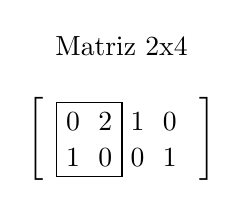
\begin{tikzpicture}[baseline=(M.center)]
 \matrix (M) [matrix of math nodes,left delimiter={[},right delimiter={]}] {
 0 & 2 & 1 & 0 \\
 1 & 0 & 0 & 1 \\
 };
 \draw (M-1-1.north west) rectangle (M-2-2.south east);
 \node[above=10pt of M.north] {Matriz 2x4};
\end{tikzpicture}
\hspace{0.8cm}\bigotimes\hspace{0.8cm}
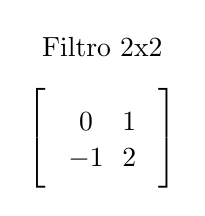
\begin{tikzpicture}[baseline=(M.center)]
 \matrix (M) [matrix of math nodes,left delimiter={[},right delimiter={]}] {
  0 & 1 \\
 -1 & 2 \\
 };
 \node[above=10pt of M.north] {Filtro 2x2};
\end{tikzpicture}
\hspace{0.8cm}=\hspace{0.8cm}
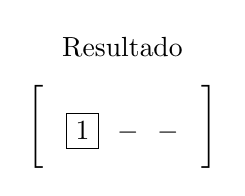
\begin{tikzpicture}[baseline=(M.center)]
 \matrix (M) [matrix of math nodes,left delimiter={[},right delimiter={]}] {
    \boxed{1} & - & - \\
 };
 \node[above=10pt of M.north] {Resultado};
\end{tikzpicture}
$$

$$
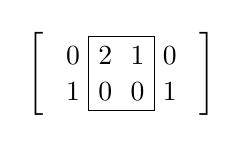
\begin{tikzpicture}[baseline=(M.center)]
 \matrix (M) [matrix of math nodes,left delimiter={[},right delimiter={]}] {
    0 & 2 & 1 & 0 \\
    1 & 0 & 0 & 1 \\
 };
 \draw (M-1-2.north west) rectangle (M-2-3.south east);
\end{tikzpicture}
\hspace{0.8cm}\bigotimes\hspace{0.8cm}
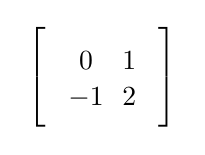
\begin{tikzpicture}[baseline=(M.center)]
 \matrix (M) [matrix of math nodes,left delimiter={[},right delimiter={]}] {
  0 & 1 \\
  -1 & 2 \\
 };
\end{tikzpicture}
\hspace{0.8cm}=\hspace{0.8cm}
\begin{bmatrix}
 1 & \boxed{1} & - \\
 \end{bmatrix}
$$

$$
\hspace{0.2cm}
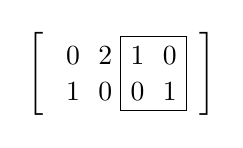
\begin{tikzpicture}[baseline=(M.center)]
 \matrix (M) [matrix of math nodes,left delimiter={[},right delimiter={]}] {
    0 & 2 & 1 & 0 \\
    1 & 0 & 0 & 1 \\
 };
 \draw (M-1-3.north west) rectangle (M-2-4.south east);
\end{tikzpicture}
\hspace{1cm}\bigotimes\hspace{0.9cm}
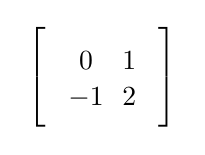
\begin{tikzpicture}[baseline=(M.center)]
 \matrix (M) [matrix of math nodes,left delimiter={[},right delimiter={]}] {
  0 & 1 \\
  -1 & 2 \\
 };
\end{tikzpicture}
\hspace{0.8cm}=\hspace{0.8cm}
\begin{bmatrix}
 1 & 1 &  \boxed{2} \\
 \end{bmatrix}
$$

\subsection*{Tamanho do passo e preenchimento}

O Tamanho do passo — ou stride — serve para especificar a distancia de pixels entre os passos da camada.  No exemplo acima esse parâmetro é definido como 1, por isso a matriz selecionada pula 1 pixel para direita entre os passos. Esse valor altera o tamanho da matriz resultante \cite{dp_overview}.

O preenchimento — ou padding — é uma técnica utilizada para manter o mesmo tamanho da entrada, adicionando bordas com zeros antes das operações da camada para ter como saída uma matriz do mesma dimensão da matriz original. Isso é usado devido a desvantagem em perder os detalhes nas bordas das imagens no processamento de uma camada \cite{dp_overview}.

\subsection*{Camada de agrupamento}

A camada de agrupamento — ou pooling — tem como tarefa primordial uma técnica para reduzir o tamanho do mapa de características, porém preservando os padrões mais relevantes. Dentre os recursos essenciais dessa camada estão o tamanho do agrupamento e a operação que será realizada. O maior problema dessa camada é pelo fato dela apenas identificar aonde essas características estão e não se tem ou não, \emph{i.e.}, dependendo de qual operação e a quantidade de camadas pode não ser possível guardar as principais características de forma integra causando uma redução no desempenho final da predição \cite{dp_overview}.

Existem vários tipos de agrupamento, os mais utilizados são: agrupamento máximo, agrupamento médio e agrupamento global médio que estão explicados abaixo em exemplos baseados em \citeonline{Alzubaidi2021}.

\subsubsection*{Agrupamento máximo}

É definido o resultado final com base no máximo encontrado pelo tamanho do agrupamento, exemplo a seguir usando um mapa de características com tamanho 4x4 e agrupamento de tamanho 2x2.

$$
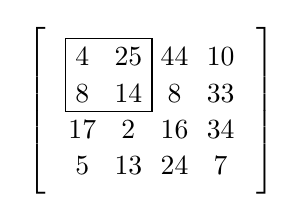
\begin{tikzpicture}[baseline=-0.5ex]
    \matrix (M) [matrix of math nodes,left delimiter={[},right delimiter={]}] {
        4 & 25 & 44 & 10\\
        8 & 14 & 8 & 33 \\
        17 & 2 & 16 & 34 \\
        5 & 13 & 24 & 7 \\
    };
    \draw (M-1-1.north west) rectangle (M-2-2.south east);
\end{tikzpicture}
= 
\begin{bmatrix}
	\boxed{25} & 44 \\
	17 & 34 \\
   \end{bmatrix}
$$

\subsubsection*{Agrupamento médio}

É definido o resultado final com base na média encontrada pelo tamanho do agrupamento, exemplo a seguir usando um mapa de características com tamanho 4x4 e agrupamento de tamanho 2x2.

$$
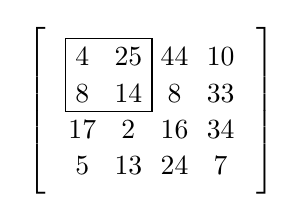
\begin{tikzpicture}[baseline=-0.5ex]
    \matrix (M) [matrix of math nodes,left delimiter={[},right delimiter={]}] {
        4 & 25 & 44 & 10\\
        8 & 14 & 8 & 33 \\
        17 & 2 & 16 & 34 \\
        5 & 13 & 24 & 7 \\
    };
    \draw (M-1-1.north west) rectangle (M-2-2.south east);
\end{tikzpicture}
= 
\begin{bmatrix}
	\boxed{12} & 23 \\
	9 & 20 \\
   \end{bmatrix}
$$

\subsubsection*{Agrupamento global médio}

É definido o resultado final com base na média geral do mapa o que sempre tem como saída uma matrix 1x1, exemplo a seguir usando um mapa de características com tamanho 4x4.

$$
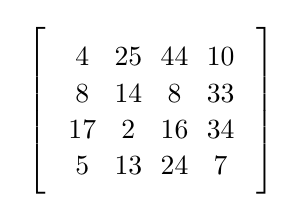
\begin{tikzpicture}[baseline=-0.5ex]
    \matrix (M) [matrix of math nodes,left delimiter={[},right delimiter={]}] {
        4 & 25 & 44 & 10\\
        8 & 14 & 8 & 33 \\
        17 & 2 & 16 & 34 \\
        5 & 13 & 24 & 7 \\
    };
\end{tikzpicture}
= 
\begin{bmatrix}
	16
   \end{bmatrix}
$$

\subsection*{Camada totalmente conectada}

A camada totalmente conectada geralmente é utilizada no final da arquitetura e cria a partir de cada neurônio uma ligação direta para cada etiqueta final. Isso torna essa camada extremamente pesada computacionalmente. O número de neurônios dessa camada é equivalente ao número de classes propostas. Além disso é quando chega nessa camada que a função de perda é calculada e se inicia a retropropagação \cite{Alzubaidi2021, computation11030052}.

\subsection*{Função de perda}
A função de perda é calculada na camada de saída e serve para mensurar o sucesso obtido comparando com fórmulas o resultado da arquitetura com o resultado real do conjunto de dados. O resultado dessa função irá ajudar na retropropagação, \emph{i.e.}, servirá para ajustar os pesos e viéses da conexão entre os neurônios para minimizar o erro. A seguir algumas funções de perda, pontuando que todo esse subtópico é baseado em 
\citeonline{Alzubaidi2021}.

\subsubsection*{Softmax ou entropia cruzada ou logarítmica}
Muito utilizada para medir a performace de uma rede neural convolucional principalmente quando o resultado final têm várias classes. Antes dessa função de perda é necessário usar a função de ativação softmax descrita na \cref{fig:grafico_softmax} pois precisa de uma saída dentro de uma distribuição de probabilidade. Sendo N o número de classes ou o número de neurônios na camada de saída.

$$H(p,y) = -\sum_{i=1}^N y_i \log(p_i)$$

\subsubsection*{Euclidiana ou erro quadrático médio}
Muito utilizada para problemas de regressão.

$$H(p,y) = \frac{1}{2N} \sum_{i=1}^N (p_i - y_i)^2$$

\subsubsection*{Hinge}
Muito utilizado para classificação binária.

$$H(p,y) = \sum_{i=1}^N max(0, m - (2y_i - 1) p_i)$$

\subsection*{Regularização}
Quando se monta uma arquitetura de redes neurais convolucional pode se chegar em três casos sendo eles: sobreajuste (overfit), subajuste (underfit) e balanceado (optimal). O sobreajuste é quando no treinamento o modelo acerta as classes porém nos testes não, isso mostra uma dificuldade em generalizar as características. Já o subajuste não consegue pontuar bem em nenhum caso mostrando que o conjunto de dados de treinamento está pequeno para detectar padrões. Por outro lado o balanceado é quando produz resultados bons tanto no conjunto de dados de treinamento quanto no de testes \cite{Alzubaidi2021, computation11030052}.

\begin{figure}[H]
	\caption{Gráficos mostrando subajuste, balanceado e sobreajuste respectivamente}
	\centering % para centralizarmos a figura
	\includegraphics[width=15cm]{figures/fittings.png} % leia abaixo
	\legend{Fonte: \citeonline{educative2022overfitting}}
	\label{fig:arquitetura_cnn}
\end{figure}

Segundo \citeonline{Alzubaidi2021} existem algumas alternativas para evitar o sobreajuste e o subajuste, dentre alguma estão:

\begin{itemize}
    \item Dropout: Muito utilizada para evitar sobreajuste pois está técnica irá desligar um neurônio aleatoriamente colocando a saída dele como zero no processo de treinamento e portanto forçara o modelo a aprender a indentificar características diferentes em outros neurônios possibilitando a generalização do modelo.
    \item Aumentar o tamanho do conjunto de dados: caso não seja possível criar ou encontrar um maior existem técnicas para aumentar artificialmente acrescentando pequenas mudanças nas imagens existentes, algumas são rotacionar, recortar e inverter horizontamente ou verticalmente.
\end{itemize}

\subsection*{Retropropagação}
De acordo com \citeonline{brilliant2023backpropagation} o algoritmo geral de retropropagação é:

\begin{enumerate}
    \item Propagação: calcular os pares de entrada-saída $(\overrightarrow{x_d}, y_d)$ — $\overrightarrow{x_d}$ é o vetor de entrada e $y_d$ a saída verdadeira — e guardar os resultados $\hat{y_d}$ — a saída encontrada no treinamento —, $a_j^k$, $o_j^k$ para cada neurônio $j$ na camada $k$, indo da camada de entrada para camada de saída.
    
    \item Retropropagação: Calcular os pares de entrada-saída $(\overrightarrow{x_d}, y_d)$, chegando na fórmula $\frac{\partial{E_d}}{\partial{w_{ij}^k}}$ que é a derivada parcial do erro total. Na representação $E_d$ é a função de perda e $w_{ij}^k$ é o peso  conectado em um neurônio de $k - 1$. Outra forma de representar é $\delta_j^k o_i^{k - 1}$ e suas variáveis são: $\delta_j^k$ representa o erro do neurônio e $o_i^{k - 1}$ representa a saída do neurônio na camada $k -1$. Essa técnica começa na camada de saída e propaga até a última camada escondida.
    
    $$ \frac{\partial{E_d}}{\partial{w_{ij}^k}} = \delta_j^k o_i^{k - 1} $$
    
    \item Combinar gradientes individuais: Uma média simples é feita com todos resultados de $\frac{\partial{E_d}}{\partial{w_{ij}^k}}$ formando assim o gradiente total representado como $\frac{\partial{E(X, \theta)}}{\partial{w_{ij}^k}}$.
    
    $$ \frac{\partial{E(X,\theta)}}{\partial{w_{ij}^k}} = \frac{1}{N} \sum_{d=1}^{N} \frac{\partial{E_d}}{\partial{w_{ij}^k}} $$
    \item Atualiza os pesos: usando $\alpha$ como taxa de aprendizado e o gradiente total $\frac{\partial{E(X, \theta)}}{\partial{w_{ij}^k}}$ temos a seguinte equação.
    
    $$ \Delta w_{ij}^k = -\alpha \frac{\partial{E(X,\theta)}}{\partial{w_{ij}^k}} $$
\end{enumerate}

Observação: basta trocar $w_{ij}^k$ para $b_{ij}^k$ — trocar o peso pelo viés — em todo algoritmo para ajustar o viés do modelo com a tecnica de retropropagação.

\subsection*{Melhorar performace}

Com base em testes de aplicações existem algumas maneiras de melhorar a qualidade do resultado final do modelo sendo elas \cite{Alzubaidi2021}:

\begin{itemize}
    \item Aumentar o conjunto de dados
    \item Aumentar o tempo de treinamento
    \item Aumentar a profundidade ou largura da arquitetura
    \item Regularizar o modelo
    \item Ajustar os hiperparâmetros
\end{itemize}
    

\subsubsubsection*{Segmentação}
\label{sec:segmentacao}

O estudo de segmentação semântica dentro da área de redes neurais convolucionais têm três principais nichos, sendo eles: segmentação semântica que é a classificação por pixel, a segmentação de instância que atribui um id para cada objeto encontrado de uma classe, e a segmentação panóptica que junta as duas anteriores para criar uma imagem semelhante a saída de segmentação semântica porém separando objetos de mesma classe sendo essa a mais recente e completa, a diferença entre esses três tipos está ilustrado na \cref{fig:segentacoes} \space\cite{dp_semantic_segmantation, lapix}.

\begin{figure}[ht]
	\caption{Tipos de segmentação em redes neurais convolucionais}
	\centering % para centralizarmos a figura
	\includegraphics[width=10cm]{figures/segmantations.png} % leia abaixo
	\legend{Fonte: \citeonline{kirillov2019panoptic}}
	\label{fig:segentacoes}
\end{figure}

\subsubsubsection*{Segmentação semântica}

A segmentação semântica começou a ter resultados satisfatórios a partir de redes totalmente convolucionais, com o objetivo de segmentar imagens classificando pixels, esse modelo descarta a camada totalmente conectada pois a saída deverá ser uma imagem e não uma classificação — isso a torna mais rápida para treinar do que as redes neurais convolucionais —, logo usa camadas deconvolucionais para transformar a matriz de características em uma imagem de qualquer dimensão na saída. A RTC criou a arquitetura chamada de salto (ou conexões) que serve para evitar perdas em camadas de agrupamento criando conexões entre camadas não consecutivas — geralmente entre camadas convolucionais e deconvolucionais — como apresentado na \cref{fig:rtc}, a arquitetura de salto evoluiu para arquitetura codificador-decodificador.
\begin{figure}[ht]
	\caption{Exemplo de arquitetura de rede totalmente convolucional}
	\centering % para centralizarmos a figura
	\includegraphics[width=10cm]{figures/redes_totalmente_convolucionais.png} % leia abaixo
	\legend{Fonte: \citeonline{dp_semantic_segmantation}}
	\label{fig:rtc}
\end{figure}

A arquitetura codificador-decodificador — ou Encoder-Decoder —, é separada em dois passos: o primeiro para convergir no mapa de características — chamado de codificador — e o segundo para reverter — chamado de decodificador — as camadas de agrupamento para aumentar a dimensão da saída, usando camadas deconvolucionais e de desagrupamento. Outra característica importante é a conexão entre camadas de mesmo nível, como por exemplo a arquitetura UNet, que foi a primeira a implementar o padrão Codificador-Decodificador. Na \cref{fig:unet} pode-se observar que tem formato da letra U, sendo a descida a parte de codificação e subida decodificação \space\cite{dp_semantic_segmantation, lapix, unetArq}.

\begin{figure}[ht]
	\caption{Arquitetura codificador-decodificador UNet}
	\centering % para centralizarmos a figura
	\includegraphics[width=10cm]{figures/unet.png} % leia abaixo
	\legend{Fonte: \citeonline{unetArq}}
	\label{fig:unet}
\end{figure}

\subsubsubsection*{Segmentação de instância}

Outro problema dentro da área de visão computacional é a detecção de objetos, a primeira solução foi com Características de regiões com RNC — Regions with CNN features (R-CNN) — que se resume em dividir a imagem de entrada em regiões de interesse e nessas regiões aplicar uma RNC. A arquitetura que seleciona essas regiões é chamada de Rede de Proposta de Região (RPR) — ou Region Proposal Network (RPN) — o que auxilia na detecção por caixas delimitadoras. Essa ideia inicial foi estendida para segmentação de instância criando também máscara nos objetos, como por exemplo a arquitetura Mask R-CNN \space\cite{dp_semantic_segmantation, lapix}.

A arquitetura Mask R-CNN é derivado do Fast R-CNN — aprimoramento do R-CNN aplicando conceito RoIPool para classificar — onde há uma segmentação de máscara em cada RoI — ou Região de interesse — paralela com a classificação da caixa delimitadora. A máscara é classificada com uma pequena RTC em cada RoI. Além de ter uma pequena melhoria na RoIPool, pois havia um problema de alinhamento nas localizações espaciais exatas, essa camada é chamada de RoIAlign \space\cite{maskRCNN}.

\subsubsubsection*{Segmentação panóptica}

Um problema encontrado na segmentação semântica é que objetos de mesma classe não são separados como na segmentação de instância, logo surgiu uma ideia para criar uma solução usando as duas técnicas. Esse conceito surgiu do trabalho \citeonline{kirillov2019panoptic} e consiste na definição geral da ideia, uma métrica — que será explicada posteriormente — unificada para classificar os resultados do modelo além de fazer a distinção entre coisas — ou stuff — que não são contáveis, como o céu e os objetos — ou things — que são contáveis como carros, pessoas, etc.
Os principais conjunto de dados para tarefa panóptica são COCO-Panoptic, Cityscapes, Mapillary Vistas, ADE20K, e Indian Driving Dataset. Cada conjunto de dados possui diversas classes para o modelo aprender \space\cite{v7labs2022panoptic}.

\subsubsubsection*{Métricas e técnicas}
\label{sec:metricas_tecnicas}

No ramo de segmentação existem diversas métricas que podem ser usadas, dentre elas algumas serão destacas nesta monografia a seguir:

\subsubsubsection*{Classificação de conjuntos}
\label{sec:classificacao_conjuntos}

A classificação de conjuntos é uma técnica para criar relações entre a imagem de predição e a imagem do conjunto de dados. Ela se divide em quatro conjuntos sendo eles: Positivo Verdadeiro — ou True Positive(TP) —
% sendo o requisito ter uma intersecção significativa entre classes iguais, \emph{i.e.}, IoU > 0.5
, Negativo Verdadeiro — ou True Negative(TN) —, Falso Positivo — ou False Positive(FP) — quando um objeto não é correspondido na imagem de predição e por fim o Falso Negativo — ou False Negatives(FN) — quando um objeto não é correspondido na imagem do conjunto de dados. Essa técnica pode ser usada em modelos de classificação binária usando uma matriz de confusão mas na área de segmentação costuma-se contar os pixeis e sua representação visual pode-se observar na \cref{fig:conjuntos} \space\cite{kirillov2019panoptic, Wang2020}.
\begin{figure}[ht]
	\caption{Exemplo da classificação dos conjuntos usados nas métricas de segmentação}
	\centering % para centralizarmos a figura
	\includegraphics[width=15cm]{figures/pan_metric.png} % leia abaixo
	\legend{Fonte: \citeonline{slidesKirillov} editado}
	\label{fig:conjuntos}
\end{figure}


\subsubsubsection*{F1 Score}

O F1 Score é uma métrica que pode ser utilizada para calcular a eficiência de modelos de segmentação de instância,  baseando-se em encontrar uma relação entre a área das classes da imagem de saída com as classes na imagem do conjunto de dados porém diminuindo o peso dos erros. Varia de 0 a 1 sendo 1 com maior eficiência. Segue a exemplificação da \cref{eq:f1} \space\cite{Chicco2020}:

\begin{equation}
	\label{eq:f1}
	F1\ Score = \frac{\text{TP}}{(TP + \frac{FP}{2} + \frac{FN}{2} )}
\end{equation}

\subsubsubsection*{Coeficiente de correlação de Matthews}

O coeficiente de correlação de Matthews — ou Matthews Correlation Coefficient (Mcc) —  é uma métrica que pode ser utilizada para mensurar a eficiência de modelos de segmentação,  baseando-se no coeficiente de correlação de Pearson. Varia de -1 a 1 sendo 1 com maior correlação, 0 inconclusivo e -1 sem correlação. Segue a exemplificação da \cref{eq:mcc} \space\cite{Chicco2020, confusion_matrix_calculator}:

\begin{equation}
	\label{eq:mcc}
	Mcc = \frac{\text{TP}\cdot\text{TN}-\text{FP}\cdot\text{FN}}{\sqrt{ (\text{TP}+\text{FP})\cdot(\text{TP}+\text{FN})\cdot(\text{TN}+\text{FP})\cdot(\text{TN}+\text{FN}) }}
\end{equation}

\subsubsubsection*{Taxa de descoberta falsa}

A taxa de descoberta falsa — ou False Discovery Rate (FDR) — é uma métrica utilizada para calcular o erro obtido na imagem de predição,  baseando-se em encontrar uma relação entre ao erro obtido, divido pelo erro mais acerto esperado. Varia de 0 a 1 sendo 1 o pior caso e 0 o melhor. Segue a exemplificação da \cref{eq:fdr} \space\cite{confusion_matrix_calculator}:

\begin{equation}
	\label{eq:fdr}
	Fdr = \frac{FP}{FP + TP}
\end{equation}


\subsubsubsection*{Taxa de Falso Negativo}

A taxa de falso negativo — ou False Negative Rate (FNR) — é uma métrica utilizada para calcular o erro obtido na imagem verdade,  baseando-se em encontrar uma relação entre ao erro obtido, divido pelo erro mais acerto esperado. Varia de 0 a 1 sendo 1 o pior caso e 0 o melhor. Segue a exemplificação da \cref{eq:fnr} \space\cite{confusion_matrix_calculator}:

\begin{equation}
	\label{eq:fnr}
	Fnr = \frac{FN}{FN + TP}
\end{equation}

\subsubsubsection*{Acurácia}

A acurácia — ou Accuracy (Acc) — é uma métrica utilizada para calcular a eficiência de modelos de segmentação semântica,  baseando-se em encontrar uma relação entre a área das classes da imagem de saída com as classes na imagem do conjunto de dados para todos conjuntos. Varia de 0 a 1 sendo 1 com maior eficiência. Segue a exemplificação da \cref{eq:acc} \space\cite{Chicco2020}:

\begin{equation}
	\label{eq:acc}
	Acc = \frac{\text{TP + TN}}{\text{(TP + TN + FP + FN)}}
\end{equation}

\subsubsubsection*{União sobre intersecção}

A união sobre intersecção — Intersection over Union (IoU) — ou índice de Jaccard é uma métrica muito utilizada para calcular a eficiência de modelos de segmentação, ela se baseia em encontrar uma relação entre a área das classes da imagem de saída com as classes na imagem do conjunto de dados para qualquer valor positivo, isto é, desconsiderando o conjunto positivo falso. Varia de 0 a 1 sendo 1 com maior eficiência. Segue a exemplificação da \cref{eq:iou} \space\cite{iou_metric_link}:

\begin{equation}
	\label{eq:iou}
	IoU = \frac{\text{TP}}{\text{(TP + FP + FN)}}
\end{equation}

\subsubsubsection*{Qualidade panóptica}

A qualidade panóptica — ou Panoptic Quality (PQ) — foi definido pela primeira vez no artigo \citeonline{kirillov2019panoptic}, e se resume na fórmula:

\begin{equation}
\label{eq:pq_metric}
PQ = \frac{\sum_{(p,g)\in TP}IoU(p,g)}{ |TP| + \frac{1}{2}|FP| + \frac{1}{2}|FN|}
\end{equation}

Multiplicando a \cref{eq:pq_metric} por $\frac{|TP|}{|TP|}$ tem-se:

\begin{equation}
	\label[]{eq:pq_metric_mult}
	PQ = \underbrace{\frac{\sum_{(p,g)\in TP}IoU(p,g)}{|TP|}}_{\text{Segmentation Quality (SQ)}}
	\times
	\underbrace{\frac{|TP|}{|TP| + \frac{1}{2}|FP| + \frac{1}{2}|FN|}}_{\text{Recognition Quality (RQ)}}
\end{equation}

Portanto pode-se concluir que PQ é apenas uma simplificação para uma fórmula que contém uma relação entre métricas de segmentação semântica e de instância.

Com base no subtópico \hyperref[sec:segmentacao]{Segmentação} percebe-se que a segmentação panóptica é a mais completa e por efeito de estudos será utilizado o mesmo para concluir o trabalho. Como nesse nicho existem várias alternativas será utilizado a métrica demonstrada na \cref{eq:pq_metric} para analisar resultados e selecionar o modelo.

\subsubsubsection*{Resultados de modelos do nicho de segmentação panóptica}

Os resultados são de uma competição em aberto criada pela Cityscapes Dataset, essa competição tem várias modalidades e esses são referentes ao nicho de segmentação panóptica utilizando a métrica PQ na classe de pessoas. A exibição dos resultados contendo a métrica PQ que classifica pessoas com os quinze melhores modelo encontra-se na \cref{tab:resultados-cityscapes} \space\cite{datasetResults}.
\begin{table}[h]
	\centering
	\caption{Top 15 modelos que melhor classificam pessoas com métrica P em segmentação panóptica}
	\label{tab:resultados-cityscapes}
	\begin{tabular}{|l|c|}
	  \hline
	  Nome do modelo & PQ (\%) \\
	  \hline
	  EfficientPS [Mapillary Vistas] & 61,6 \\
	  EfficientPS [Cityscapes-fine] & 60,9 \\
	  Panoptic-DeepLab w/ SWideRNet [Mapillary Vistas + Pseudo-labels] & 60,6 \\
	  hri\_panoptic & 60,6 \\
	  Naive-Student (iterative semi-supervised learning with Panoptic-DeepLab) & 60,2 \\
	  Panoptic-DeepLab w/ SWideRNet [Mapillary Vistas] & 59,8 \\
	  iFLYTEK-CV & 59,2 \\
	  Panoptic-DeepLab [Mapillary Vistas] & 58,5 \\
	  Panoptic-DeepLab w/ SWideRNet [Cityscapes-fine] & 58,4 \\
	  Seamless Scene Segmentation & 57,7 \\
	  Axial-DeepLab-XL [Mapillary Vistas] & 57,2 \\
	  Unifying Training and Inference for Panoptic Segmentation [COCO] & 56,5 \\
	  kMaX-DeepLab [Cityscapes-fine] & 56 \\
	  Axial-DeepLab-L [Mapillary Vistas] & 55,9 \\
	  TASCNet-enhanced & 55,2 \\
	  \hline
	\end{tabular}
  \end{table}





\subsubsubsection*{EfficientPS}
\label{sec:EfficientPS}

EfficientPS é uma solução eficiente para a segmentação panóptica, proposta no artigo \citeonline{mohan2020efficientps}. Em seu repositório na internet \citeonline{efficientpsGit}, há algumas recomendações de tecnologias utilizadas para desenvolver e testar o modelo. Embora possa funcionar em outros cenários, não há suporte dos criadores para tais aplicações. Essas tecnologias são: uma distribuição de sistema operacional\footnote{Programa que gerencia a parte física de um computador; meio termo entre o usuário e a parte física do computador.} com núcleo Linux, conforme descrito em \citeonline{redhat2023}; a linguagem de programação Python na versão 3.7, que, segundo \citeonline{analyticsindiamag2023}, é amplamente utilizada no campo da IA devido à sua simplicidade e às diversas bibliotecas que facilitam a criação de modelos complexos; o PyTorch na versão 1.7, que, de acordo com \citeonline{pytorch2023}, é uma estrutura baseada na biblioteca Torch, visando facilitar a criação de modelos de aprendizado profundo; o CUDA Toolkit na versão 10.2, que, segundo \citeonline{cudatoolkit2023}, é uma biblioteca para proporcionar aceleração do processamento com placas de vídeo da marca Nvidia; e, por fim, o GCC nas versões 7 ou 8, que, conforme \citeonline{gcc2023}, é um compilador das linguagens C e C++, frequentemente utilizados em bibliotecas Python, como o PyTorch, por exemplo.

\subsubsubsection*{Arquitetura}

O artigo apresenta uma arquitetura que se inicia com um \textit{backbone} — parte responsável por identificar características —, utilizando uma Rede de Pirâmide de Características (RPC)\footnote{Estrutura de pirâmide para extrair características em várias escalas de uma imagem \space\cite{piramide}} de dois caminhos, seguida de dois cabeçotes paralelos: um para uma arquitetura de segmentação semântica, de autoria própria, e outro de instância, com modificações baseadas na topologia Mask R-CNN. Finalmente, a saída dos dois cabeçotes é combinada no módulo de fusão panóptica para gerar a saída final com a imagem de segmentação panóptica. Esta arquitetura é ilustrada na \cref{fig:arqEP}.

\begin{figure}[ht]
	\caption{Arquitetura geral do EfficientPS}
	\centering % para centralizarmos a figura
	\includegraphics[width=15cm]{figures/arqEP.png} % leia abaixo
	\legend{Fonte: \citeonline{mohan2020efficientps}}
	\label{fig:arqEP}
\end{figure}

\subsubsubsection*{Backbone da rede}

A espinha dorsal — ou backbone — consiste em uma codificação combinada a uma bifurcação paralela usando RPC. O codificador é essencial para arquiteturas de segmentação e, para melhorar a capacidade de representação, é necessário aumentar o número de parâmetros e a complexidade. No entanto, neste artigo, os autores apresentam uma solução equilibrada neste aspecto. O codificador contém nove blocos (em vermelho), mostrados na \cref{fig:arqEP}, e as saídas 2º, 3º, 5º e 9º — da esquerda para a direita — correspondem aos fatores de redução de amostragem x4, x8, x16 e x32, respectivamente. Essas saídas se conectam à bifurcação paralela, que possui sentidos opostos, para gerar mais detecções de características. Posteriormente, é realizada uma combinação entre camadas de mesma dimensão, utilizando camadas de convolução separável em profundidade — que divide em etapas espaciais e de canal, aplicadas a cada canal e a cada pixel de saída, respectivamente —, resultando nas saídas \( P_4 + P_8 + P_{16} + P_{32} \) \cite{mohan2020efficientps, redes-neurais-convolucionais-separaveis-em-profundidade}.

\subsubsubsection*{Cabeçote de Segmentação Semântica}

O cabeçote de segmentação semântica, uma criação dos autores, é dividido em três módulos: o Extrator de Características em Larga Escala (ECLE) — ou Large Scale Feature Extractor (LSFE) —, destinado a capturar recursos finos em larga escala de forma eficiente; o módulo DPC, que deve ser capaz de capturar contexto de longo alcance, mas em pequena escala; e o módulo MC, responsável por mitigar a incompatibilidade entre recursos de grande e pequena escala nas camadas de agregação \cite{mohan2020efficientps}.

As quatro entradas do cabeçote, \( P_4 + P_8 + P_{16} + P_{32} \), são processadas separadamente. As entradas \( P_{16} + P_{32} \) — de pequena escala — alimentam dois módulos DPC paralelos, enquanto \( P_4 + P_8 \) — de larga escala — alimentam dois módulos ECLE paralelos \cite{mohan2020efficientps}.


\subsubsubsection*{Cabeçote de segmentação de instância}

Este cabeçote é derivado da arquitetura Mask R-CNN, e as modificações realizadas foram três: a substituição da convolução padrão por convolução separável em profundidade — para reduzir o número de parâmetros consumidos pela rede —, a substituição da camada de normalização em lote por iABN Sync\footnote{Normalização em lotes entre cores de GPU para aumentar o desempenho.} e a troca da função ReLU, definida em \cref{eq:relu_func}, pela função Leaky ReLU, definida em \cref{eq:relu_leaky_func} \cite{mohan2020efficientps, redes-neurais-convolucionais-separaveis-em-profundidade, serp-ai}.

\subsubsubsection*{Módulo de fusão panóptica}

O módulo de fusão panóptica é essencial para construir a imagem com segmentação panóptica. Nesta etapa, os resultados dos dois cabeçotes anteriormente explicados são combinados. Esta tarefa não é simples, pois requer uma lógica sofisticada para lidar com as sobreposições encontradas. O módulo foi projetado para ser adaptativo e usar as duas entradas de forma equivalente \cite{mohan2020efficientps}.

Resumidamente, o módulo aplica técnicas para reduzir o número de instâncias baseando-se na métrica logística — um valor numérico que pontua a confiança. Ele realiza agregações entre os resultados dos dois cabeçotes e desenha com fundo preto as instâncias de maior confiança. Posteriormente, preenche com a parte de \textit{stuff} — classes semânticas de menor importância — da entrada semântica \cite{mohan2020efficientps}.


\section{Trabalhos relacionados}

Esta seção destina-se a análise e discussão da metodologia e dos resultados prospostos por \citeonline{geracao_procedural_jogos_2d,kirillov2019panoptic}. 

\subsection*{Geração Procedural de Mapas para Jogos 2D}

No trabalho \citeonline{geracao_procedural_jogos_2d}, é apresentado uma solução simples para criar mapas de cavernas, calabouços e ilhas para jogos 2D. O algoritmo foi dividido em três partes sendo elas: geração recursiva de terrenos, validação de tamanho e correção da coesão. Os autores concluíram que não existe literatura sobre geração procedural de salas diversas e corredores distintos como o algoritmo proposto. Sugerem duas possibilidades para trabalhos futuros sendo elas: usar algoritmos genéticos para mensurar a qualidade dos mapas gerados e promover pela seleção natural e a outra possibilidade é mesclar o algoritmo proposto com técnicas de geração de salas interligadas por corredores, de forma a possibilitar a criação de mapas com algumas salas pré-definidas inseridas em um mapa aberto contínuo.

\subsection*{Panoptic Segmentation}

No trabalho \citeonline{kirillov2019panoptic} é definido a ideia geral de segmentação panóptica além de definir conceitos importantes como coisas e objetos e a métrica unificada para medir o desempenho de modelos dessa área. Também é feito alguns testes comparando resultados humanos com um modelo simples proposto com eles combinando PSPNet e Mask R-CNN usando a métrica de qualidade panóptica definida por eles. Os resultados mostraram a superioridade humana na segmentação panóptica em três conjuntos de dados diferentes, sendo eles: Cityscapes, ADE20k e Vistas, as métricas usadas foram qualidade panóptica, qualidade semântica, qualidade de reconhecimento, qualidade panóptica
 de coisas e qualidade panóptica de objetos. O melhor resultado para a máquina em comparação com o humano foi no conjunto de dados Cityscapes avaliando a qualidade semântica, sendo 84,1 para o humano e 80,9 para máquina. O pior resultado para a máquina em relação ao humano foi no conjunto de dados ADE20k na qualidade panóptica de coisas, sendo 71,0 para os humanos e 24,5 para a máquina.

 \subsection*{Polygonal Map Generation for Games}

 No artigo de \citeonline{amitp2010} é apresentado toda uma jornada de desenvolvimento de um algoritmo de geração procedural de conteúdo, é mostrando as técnicas para gerar o mapa com o diagrama de Voronoi, gerar os rios e biomas utilizando as camadas de elevação e umidade do polígono e a aplicando isso no diagrama de Whittaker para definir o bioma do polígono. Também é apresentado uma técnica para adicionar ruídos nas arestas dos políginos fazendo com que o mapa se torne mais orgânico e realista.

\chapter{Desenvolvimento}

Neste capítulo é apresentada a descrição da proposta e relatado o processo de
desenvolvimento e avaliação da implementação.

\section{Proposta}

Este trabalho propõe a criação de um protótipo destinado a gerar um mapa de forma procedural, cujo contorno é selecionado a partir de uma imagem processada por um modelo de segmentação panóptica \footnote{No resultado apenas será identificado os pixeis de classes contidas nos conjuntos de dados escolhidos, e todos citados no capítulo 2 são de contexto urbano}. O mapa resultante replicará o contorno da seleção em 2D e 3D.

A \cref{fig:etapas_proposta} apresenta os passos dessa abordagem, onde a imagem a representa a entrada para o processo de segmentação panóptica, e a imagem b é o resultado desse processo. O modelo utilizado para a segmentação panóptica é o EfficientPS, conforme detalhado no subtópico \hyperref[sec:EfficientPS]{EfficientPS}, e pode ser encontrado no GitHub dos próprios autores \citeonline{mohan2020efficientps}. Após a segmentação da imagem, o usuário terá a capacidade de selecionar um contorno, resultando em uma máscara binária, conforme ilustrado na imagem c, que representa a escolha do segmento, como, por exemplo, o carro amarelo da imagem b. Subsequentemente, um mapa procedural será gerado com o contorno escolhido, conforme evidenciado na imagem d. Essa representação incluirá uma sobreposição do contorno do veículo, meramente para ilustrar que a ilha gerada terá um contorno semelhante. As cores na representação indicam o oceano (azul), a floresta (verde) e as montanhas (cinza). Além disso, será automatizado para atualizar o relevo de um mapa em 3D.

% footnote?
%
% Após a segmentação da imagem — como ilustra a \cref{fig:segmantations_2} — o usuário poderá selecionar uma das áreas coloridas da imagem que será utilizada para gerar a ilha.

% Em seguida será criado um diagrama de Voronoi (pode ser observado na \cref{fig:diagrama_voronoi}), esse diagrama será utilizado para marcar a localização da ilha, assim gerando o mapa e os biomas a partir da atribuição de propriedades para cada ponto, polígono e reta do diagrama.

% O resultado esperado pode ser contemplado na \cref{fig:resultado_geracao}, onde o azul representa o oceano, o verde retrata a floresta e o cinza caracteriza uma montanha.


\begin{figure}[!ht]
	\centering
    \caption{Etapas da proposta}
	\includegraphics[width=0.9\textwidth]{figures/etapas_proposta.png}
    \legend{Fonte: \citeonline{kirillov2019panoptic}}
	\label{fig:etapas_proposta}
\end{figure}


% \begin{figure}[!ht]
% 	\centering
%     \caption{Imagem de entrada para rede neural.}
% 	\includegraphics[width=0.6\textwidth]{figures/segmantations_1.png}
%     \legend{Fonte: \citeonline{kirillov2019panoptic}}
% 	\label{fig:segmantations_1}
% \end{figure}

% \begin{figure}[!ht]
% 	\centering
%     \caption{Imagem saída de um modelo de segmentação panóptica.}
% 	\includegraphics[width=0.6\textwidth]{figures/segmantations_2.png}
%     \legend{Fonte: \citeonline{kirillov2019panoptic}}
% 	\label{fig:segmantations_2}
% \end{figure}

% \begin{figure}[!ht]
% 	\centering
%     \caption{Ilha gerada a partir da segmentação panóptica e aplicando um filtro com o diagrama de Voronoi, azul representa oceano, verde floresta, cinza montanhas.}
% 	\includegraphics[width=0.6\textwidth]{figures/segmantations_pnl.png}
%     \legend{Fonte: Criação própria}
% 	\label{fig:resultado_geracao}
% \end{figure}



\section{Implementação}

Pode-se dividir a implementação em quatro partes, sendo elas: segmentar imagens, selecionar contorno, gerar proceduralmente o mapa com biomas e interligar as ferramentas atráves de uma interface gráfica.

\subsection{Segmentar imagens}

A segmentação da imagem é usada para classificar os pixels da imagem a partir de padrões reconhecidos por uma inteligência artificial. A partir disso é possível o usuário selecionar o contorno para gerar o mapa.

A linguagem de programação utilizada para desenvolvimento do projeto foi Python pois existem muitas bibliotecas que auxiliam na criação de arquiteturas complexas de Inteligência Artificial como o \hyperref[sec:EfficientPS]{EfficientPS}.

Utilizou-se o código aberto oficial do trabalho ciéntifico postado no repositório do Github \footnote{\url{https://github.com/DeepSceneSeg/EfficientPS}}.

Percebe-se que o resultado do modelo proposto não foi o esperado pois objetos de mesma classe como carros tem a mesma cor com uma borda branca exemplificados na \cref{fig:resultado_inicial}. Logo tentou-se mudar o código para gerar uma saída com objetos de mesma classe com cores diferentes como na figura \cref{fig:segmantations_2}.

\begin{figure}[!ht]
	\centering
    \caption{Resultado inicial do repositório.}
	\includegraphics[width=0.6\textwidth]{figures/resultado_primario.png}
    \legend{Fonte: Criação própria}
	\label{fig:resultado_inicial}
\end{figure}

Seguiu-se os passos citados numa publicação no repositório \footnote{\url{https://github.com/DeepSceneSeg/EfficientPS/issues/23}} porém o resultado obtido não foi satisfatório pois não possível discernir quais segmentos pertenciam as respectivas classes, o resultado é ilustrado na \cref{fig:resultado_obtido}.

\begin{figure}[!ht]
	\centering
    \caption{Resultado obtido seguindo os passos da publicação no repositório.}
	\includegraphics[width=0.6\textwidth]{figures/resultado_obtido.png}
    \legend{Fonte: Criação própria}
	\label{fig:resultado_obtido}
\end{figure}

\subsection{Selecionar contorno}

Para representar a seleção do contorno utilizou-se uma técnica chamada de imagem binária, explicaa no subtópico seguinte.

\subsubsection{Imagem binária}

Uma imagem  binária contém  apenas duas cores, geralmente preto e  branco e para essa aplicação sera utilizado como uma máscara para servir de auxilio ao  gerar o  mapa no contorno desejado \cite{Aznag2020}.

Utilizou-se duas maneiras para selecionar o contorno, sendo eles: selecionar por cor, selecionar por preenchimento por inundação — ou  em inglês  flood fill —.

\subsubsubsection*{Selecionar por cor}

O metódo de selecionar por cor se baseia em pegar a cor específica do clique na imagem e percorrer a imagem comparando a cor alvo com a cor da imagem, caso seja a mesma pinte o mesmo pixel da nova imagem como branco e caso não seja pinte como preto.

\subsubsubsection*{Selecionar por preenchimento de inundação}

O método de  selecionar por preenchimento por inundação é um algoritmo de expansão a partir de um pixel validando se contém a mesma cor.

A implementação inicia uma matriz de zeros com tamanho 2 pixeis maior do que a imagem original.

O clique na  imagem será a semente — ou em inglês  seed — e a partir disso o algoritmo começa uma expansão para os pixeis vizinhos — de cima, baixo, esquerda e direita — caso contenha o mesmo valor de cor pinta de cor branca, e refaz com os pixels marcados  anteriormente.

\subsubsubsection*{Tratamento da  imagem binária}

Após a saída dos algoritmos de seleção, o objeto selecionado é detectado e centralizado em uma nova imagem, depois recortamos e redimensionamos a partir do centro de forma que fique quadrada. Todos os passos são observáveis na \cref{fig:saidas_selecao}.

\begin{figure}[!ht]
	\centering
    \caption{Passos da seleção da saída da inteligência  artificial.}
	\includegraphics[width=0.6\textwidth]{figures/saidas_selecao.png}
    \legend{Fonte: \space Autoria própria}
	\label{fig:saidas_selecao}
\end{figure}

\subsection{Geração procedural do mapa}

Usou-se como base para a geração procedural do mapa o artigo \hyperref[sec:geracaoProcedural]{Polygonal Map Generation for Games} com uma implementação não oficial porém baseada no artigo feito em Python.

\subsubsection{Ilha gerada no contorno}

Para gerar o mapa da ilha é preciso gerar um diagrama de Voronoi. No diagrama primeiro é definido os pontos de quantidade preestabelecida e de localização pseudo-aleatória, esses pontos serão os centroides dos polígonos. Os vértices dos polígonos são gerados a partir da intersecção entre retas perpendiculares aos pontos médios entre os nós vizinhos, logo é criado outro grafo com esses pontos. A definição dos vértices é ilustrada na \cref{fig:explicacao_vertice}, sendo os pontos vermelhos os centroides que são ligados por linhas pretas para gerar pontos médios, representados por pontos amarelos para traçar uma reta perpendicular, depois é calculado a intersecção representado pelo ponto azul que se torna o vertice, e a cor rosa representa a aresta do polígono.

A \cref{fig:diagrama_voronoi_pontos} ilustra o modelo do diagrama de Voronoi do algoritmo, sendo os pontos vermelhos os centroides que são ligados por linhas pretas, os pontos azuis são os vértices que se ligam com linha branca para tornar as arestas formando assim o polígono.


\begin{figure}[!ht]
	\centering
    \caption{Ilustração do cálculo para definir a localização dos vértices.}
	\includegraphics[width=0.6\textwidth]{figures/explicacao_vertice.png}
    \legend{Fonte: \space Autoria própria}
	\label{fig:explicacao_vertice}
\end{figure}

\begin{figure}[!ht]
	\centering
    \caption{Ilustração do diagrama de Voronoi.}
	\includegraphics[width=0.6\textwidth]{figures/diagrama_voronoi_pontos.png}
    \legend{Fonte: \space Autoria própria}
	\label{fig:diagrama_voronoi_pontos}
\end{figure}

\subsubsection{Mapa de altura}

\subsubsection{Testes}

Será feito um teste baseado no sutópico \hyperref[sec:uniaoSobInterseccao]{união sob intersecção} no qual irá comparar duas imagens binárias da entrada do algoritmo de geração procedural e a saída, metrificando a semelhança obtida do contorno desejado. Portanto quanto maior essa medida maior a compatibilidade com o contorno inicialmente proposto.

\subsection{Interface gráfica}

Utilizou-se a biblioteca PyQt5 para criar uma interface gráfica na qual o usuário poderá interagir e criar um mapa a partir da seleção do contorno detectado pelo modelo de IA.

Esse módulo é responsável para conectar todas as partes e obter o mapa. Portanto é necessário abrir uma imagem do diretório local, carregar e disparar a execução do processo de segmentação de imagem. Após o resultado da IA, permitir a seleção do contorno,  criar uma imagem binária a partir do contorno e envia-lá como argumento na geração procedural de mapas.

Além disso para promever a usabilidade utilizou-se um loading específico para PyQt5 e para isso teve-se que usar threads, criando classes para rodar as tarefas de forma separada e síncrona.

\chapter{Resultados}

Neste capítulo é apresentada os resultados obtidos da implementação e discutido o  impacto e possíveis causas.

\section{Apresentação}

Para apresentar os resultados, serão abordadas tabelas contendo testes com todas as combinações de imagens, uma imagem com os resultados finais das tabelas, além de uma imagem com todos os passos da aplicação.

A Tabela \ref{tab:final_input_output_2d} apresenta os resultados comparativos entre a imagem de entrada e o mapa 2D. Esta comparação é realizada utilizando a técnica de classificação de conjuntos, conforme definido por \cite{kirillov2019panoptic}. A análise foca na avaliação das métricas, conforme o número de pontos no diagrama de Voronoi, incluindo União sobre Interseção (IoU), Acurácia (Acc), F1 Score (F1), Coeficiente de Correlação de Matthews (MCC), Taxa de Descoberta Falsa (FDR), Taxa de Falso Negativo (FNR) e o tempo de execução do código \cite{Chicco2020, confusion_matrix_calculator, iou_metric_link}.

Esta tabela é crucial, pois ela evidencia, com base em dados concretos, a semelhança do mapa 2D com o contorno do mapa de entrada. Além disso, corrobora a hipótese de que um maior número de pontos no mapa leva a melhores resultados nas métricas de IoU, Acc, F1 e MCC (onde valores mais altos indicam melhor desempenho), e simultaneamente, a uma redução nos índices de FDR e FNR (onde valores menores são preferíveis, visto que representam menor erro). Observa-se, ainda, que um aumento no número de pontos implica em um maior tempo de processamento na geração procedural do mapa.

\begin{table}[h]
	\centering
	\caption{Resultados dos testes entre imagem de entrada e mapa 2d}
	\label{tab:final_input_output_2d}
	\begin{tabular}{|c|c|c|c|c|c|c|c|}
		\hline
						Pontos & IoU & Acc & F1 & MCC & FDR & FNR & Duração \\
		\hline
		50 & 0.71361 & 0.86085 & 0.8323 & 0.74079 & 0.2762 & 0.01923 & 5.33293\\
100 & 0.80033 & 0.9151 & 0.88857 & 0.82809 & 0.17938 & 0.0292 & 10.0857\\
150 & 0.83825 & 0.93506 & 0.91168 & 0.86398 & 0.13792 & 0.03125 & 15.32477\\
200 & 0.85695 & 0.94434 & 0.92268 & 0.88059 & 0.10822 & 0.04269 & 20.22667\\
250 & 0.868 & 0.94946 & 0.92908 & 0.89029 & 0.09454 & 0.04525 & 27.26459\\
300 & 0.87405 & 0.95241 & 0.93263 & 0.89612 & 0.08326 & 0.04984 & 33.46705\\
		\hline
	\end{tabular}
\end{table}


Os resultados obtidos na \cref{tab:final_input_output_3d} derivam da comparação entre a imagem de entrada e o mapa de altura, utilizando a técnica de classificação de conjuntos conforme definida por \cite{kirillov2019panoptic}. Essa comparação foi realizada para mensurar diversos aspectos, incluindo as métricas associadas ao número de pontos no diagrama de Voronoi. As métricas abrangem União sobre Interseção (IoU), Acurácia (Acc), F1 Score (F1), Coeficiente de Correlação de Matthews (MCC), Taxa de Descoberta Falsa (FDR), Taxa de Falso Negativo (FNR) e a duração da execução do código \cite{Chicco2020, confusion_matrix_calculator, iou_metric_link}.

A relevância dessa tabela reside na capacidade de demonstrar, por meio de dados concretos, a proximidade entre o mapa de altura e o contorno do mapa de entrada. Além disso, ela valida a hipótese de que o aumento no número de pontos resulta em melhores desempenhos nas métricas de IoU, Acc, F1 e MCC, indicando uma maior semelhança entre os mapas. Simultaneamente, observa-se uma diminuição nas métricas de FDR e FNR, evidenciando uma redução nos erros. Vale notar que a quantidade de pontos também impacta diretamente na duração da geração procedural do mapa, sendo um fator relevante a ser considerado.


\begin{table}[h]
	\centering
	\caption{Resultados dos testes entre imagem de entrada e mapa de altura}
	\label{tab:final_input_output_3d}
	\begin{tabular}{|c|c|c|c|c|c|c|c|}
		\hline
						Pontos & IoU & Acc & F1 & MCC & FDR & FNR & Duração \\
		\hline
		50 & 0.67955 & 0.83753 & 0.80827 & 0.70471 & 0.31036 & 0.02058 & 5.29547\\
100 & 0.74929 & 0.88637 & 0.85581 & 0.77953 & 0.23518 & 0.02501 & 9.822\\
150 & 0.79092 & 0.91133 & 0.88236 & 0.82054 & 0.18669 & 0.0319 & 15.43131\\
200 & 0.80368 & 0.91818 & 0.89056 & 0.83234 & 0.17252 & 0.03302 & 21.06372\\
250 & 0.82316 & 0.92831 & 0.90248 & 0.85016 & 0.14821 & 0.03784 & 25.92615\\
300 & 0.82598 & 0.93022 & 0.90415 & 0.85286 & 0.14182 & 0.04223 & 32.75651\\
		\hline
	\end{tabular}
\end{table}

A tabela referenciada como \cref{tab:final_output_2d_output_3d} apresenta os resultados comparativos entre o mapa de altura e sua representação em mapa 2D. Esta comparação é realizada através do método de classificação de conjuntos proposto por \cite{kirillov2019panoptic}, avaliando os resultados com base em várias métricas conforme a quantidade de pontos no diagrama de Voronoi. As métricas avaliadas incluem União sobre Interseção (IoU), Acurácia (Acc), F1 Score (F1), Coeficiente de Correlação de Matthews (MCC), Taxa de Descoberta Falsa (FDR), Taxa de Falso Negativo (FNR) e o tempo de execução do código \cite{Chicco2020, confusion_matrix_calculator, iou_metric_link}. Esta tabela é crucial para demonstrar que o mapa de altura, que se transformará no mapa 3D, assemelha-se ao mapa 2D. Essa similaridade é fundamental no protótipo do Unity para a localização do personagem, combinando o mapa 2D como minimapa e o mapa 3D com dimensão e profundidade. Observa-se também que um aumento no número de pontos resulta em maior tempo de geração procedural do mapa.


\begin{table}[h]
	\centering
	\caption{Resultados dos testes entre mapa 2d e mapa de altura}
	\label{tab:final_output_2d_output_3d}
	\begin{tabular}{|c|c|c|c|c|c|c|c|}
		\hline
						Pontos & IoU & Acc & F1 & MCC & FDR & FNR & Duração \\
		\hline
		50 & 0.91515 & 0.9589 & 0.95559 & 0.91721 & 0.06528 & 0.0222 & 5.0949\\
100 & 0.90352 & 0.95708 & 0.94924 & 0.91312 & 0.08082 & 0.01838 & 10.08713\\
150 & 0.90342 & 0.9592 & 0.94915 & 0.91636 & 0.08265 & 0.01631 & 14.82656\\
200 & 0.90421 & 0.96087 & 0.94955 & 0.91901 & 0.08312 & 0.01487 & 20.51247\\
250 & 0.90505 & 0.96207 & 0.95004 & 0.92088 & 0.08284 & 0.0142 & 26.63407\\
300 & 0.90357 & 0.96252 & 0.94921 & 0.92112 & 0.08565 & 0.01276 & 33.59293\\
		\hline
	\end{tabular}
\end{table}

A \cref{fig:result_final} contém a ilustração da classificação dos conjuntos de cada combinação. Assim, a imagem (a) ilustra a última execução da combinação entre a imagem de entrada e o mapa 2D, conforme os resultados da \cref{tab:final_input_output_2d}. A imagem (b) exibe a última execução da combinação entre a imagem de entrada e o mapa de altura, conforme os resultados da \cref{tab:final_input_output_3d}. Já a imagem (c) apresenta a última execução da combinação entre o mapa de altura e o mapa 2D, conforme os resultados da \cref{tab:final_output_2d_output_3d}.

\begin{figure}[!ht]
	\centering
    \caption{Resultados da última execução de cada combinação de imagens.}
	\includegraphics[width=\textwidth]{figures/comb_results_final.png}
    \legend{Fonte: \space Autoria própria}
	\label{fig:result_final}
\end{figure}

A \cref{fig:combs_result} apresenta todos os passos da execução do programa gerado em Python. A imagem (a) mostra uma captura de tela da interface gráfica com PyQt5. A imagem (b) exibe uma captura de tela do processo de abertura de uma imagem para segmentação. Na imagem (c), é apresentada uma captura de tela da execução do modelo EfficientPS na imagem selecionada. A imagem (d) mostra uma captura de tela da saída da segmentação panóptica pelo modelo EfficientPS. Na imagem (e), temos o carregamento pós-seleção do usuário, que, no caso, selecionou um carro com o método de preenchimento por inundação. A imagem (f) exibe o resultado do mapa 2D com o contorno selecionado anteriormente. Na imagem (g), é apresentada uma captura de tela da automação usando Unity para atualizar um terreno com o mapa de altura resultante da geração procedural. Por fim, a imagem (h) mostra uma captura de tela do Unity rodando a aplicação e abrindo o minimapa (usando o mapa 2D) para oferecer uma noção de localização no mapa 3D, usando um ponto para marcar a localização atual do personagem no minimapa (mapa 2d).


\begin{figure}[!ht]
	\centering
    \caption{Passos do programa final.}
	\includegraphics[width=\textwidth]{figures/result_final.png}
    \legend{Fonte: \space Autoria própria}
	\label{fig:combs_result}
\end{figure}

\newpage

\begin{figure}[!ht]
	\centering
    \caption{Passos do programa final utilizando o preenchimento por inundação.}
	\includegraphics[width=\textwidth]{figures/geracao_balde_tinta.png}
    \legend{Fonte: \space Autoria própria}
	\label{fig:combs_result_2}
\end{figure}

\pagebreak

Na figura \cref{fig:combs_result_2}, são delineados os mesmos estágios exibidos na figura \cref{fig:combs_result}, acrescidos de um componente relacionado ao método de reenchimento por inundação. A imagem 'a' representa a interface inicial, 'b' denota a seleção de uma imagem pelo usuário via o seletor de arquivos, 'c' ilustra a imagem escolhida pelo usuário, carregada na memória e apresentada na interface, 'd' exibe uma interface de carregamento para o processamento da geração do mapa, 'e' revela o resultado do processamento, apresentado na interface, 'f' apresenta o mapa 3D no Unity visto de cima, com o formato da ilha, e, finalmente, 'g' mostra o mapa 2D gerado, apresentado como um minimapa no mapa 3D no Unity.

\section{Análise dos resultados}

Com dos dados e observações da \cref{tab:final_input_output_2d} e da \cref{tab:final_input_output_3d} é possível afirmar que a hipótese inicial se concluiu, pois quanto mais pontos o diagrama de Voronoi tiver maior será a compatibilidade com o contorno. É possível afirmar isso devido a tendência entre as métricas dessas duas tabelas, as métricas IoU, Acc, F1 e MCC aumentam a cada linha e as métricas FDR  e FNR diminuem o erro encontrado. Outra métrica importante é a duração da geração procedural que quanto mais pontos maior a duração em segundos. Portanto deve-se analisar o cenário para o processamento e qual o melhor custo benefício.

O resultado satisfatório se comprova nas ilustrações da última execução — com 300 pontos — de cada combinação de imagens nas \cref{fig:combs_result}, percebe-se que os erros ilustrados com cores vermelha e verde são poucos e os acertos em branco e cinza prevalecem na grande maioria da imagem.

Além disso a \cref{tab:final_output_2d_output_3d} mostra-se com as observações que se mantém a confiabilidade entre a imagem 2d (minimapa) e o mapa de altura (que formará o mapa 3d) para que possa ter a funcionalidade de localização em tempo real dentro da execução do jogo.

% destacar com logica que a duração maior é para criar o grafo com os biomas e que gerar os mapas é a parte que demora pouco

%  explicar comparando em relação a cada métricas
% Tipo, esse teste foi melhor a acurácia pq...

\chapter{Considerações finais}

Neste capítulo é desenvolvido as conclusões do trabalho e trabalhos futuros para evoluir com a ciência na tentativa de conseguir resultados melhores.

\section{Conclusão}

A presente monografia aborda uma solução que viabiliza a criação de mapas 2D e 3D a partir de contornos de dois contextos distintos: uma imagem de um desenho, utilizando seleção por preenchimento por inundação, e uma imagem urbana, empregando segmentação panóptica. A implementação do projeto compreende seis fases distintas: a primeira fase concentra-se na segmentação de imagens; a segunda, na seleção de contornos; a terceira fase envolve a geração procedural de mapas com biomas variados; a quarta etapa consiste no desenvolvimento de testes para avaliar a eficácia da geração procedural; a quinta fase aborda a análise de casos de pós-processamento; e, por fim, a sexta etapa concentra-se na integração das ferramentas mencionadas por meio de uma interface gráfica intuitiva.

Os trabalhos relacionados desempenharam um papel crucial para a conclusão desta monografia. A contribuição de Kirillov (2019) foi essencial para o entendimento e a base da segmentação panóptica, que combina a segmentação de instância e semântica, além de fornecer fundamentos para a técnica de classificação de conjuntos, permitindo a utilização de métricas para validar a hipótese inicial. O modelo eficiente de segmentação panóptica descrito por Mohan et al. (2020) foi utilizado para segmentar as imagens e selecioná-las, viabilizando a criação procedural de mapas para jogos, conforme descrito por Amit (2010), com o contorno escolhido.

A fundamentação teórica proporcionada pelos trabalhos relacionados possibilitou a construção do protótipo e a execução dos testes propostos. Além disso, a proposta inicial foi comprovada, indicando que um aumento nos pontos do diagrama de Voronoi para a geração procedural do mapa resulta em uma maior aproximação do contorno da ilha gerado a partir das técnicas de segmentação.

Conclui-se que todos os objetivos propostos foram alcançados de maneira satisfatória, obtendo resultados positivos em ambos os cenários. A diversificação e personalização dos ambientes virtuais promovem um impacto positivo na experiência do jogador. Contudo, é importante ressaltar que a relação entre a adição de mais pontos e a melhoria dos resultados, juntamente com o tempo de execução, pode apresentar desafios em dispositivos com capacidades de processamento inferiores. Além disso, a dependência da biblioteca CUDA Toolkit na implementação da inteligência artificial pode limitar sua aplicabilidade em cenários menos ideais.

Nesse contexto, sugere-se a possibilidade de aprimorar a proposta utilizando algoritmos mais eficientes e multiplataforma, ampliando assim a funcionalidade para um público mais abrangente. A automação para Unity revela-se versátil, podendo ser adotada por desenvolvedores para a criação rápida de esboços de mapas 2D/3D ou como funcionalidade para consumidores de jogos, permitindo a geração de mapas a partir de contornos selecionados em fotos segmentadas.


\section{Trabalhos Futuros}

As seguintes propostas podem ser estudadas e aplicadas para aprimorar os resultados obtidos:

\begin{itemize}
    \item Utilizar um modelo de segmentação panóptica com suporte multiplataforma.
    \item Empregar paralelismo para otimizar o tempo de execução.
    \item Aplicar rasterização para aprimorar o tempo de execução.
    \item Testar o tempo de execução com outros métodos de geração procedural, visando criar um mapa baseado em um contorno.
\end{itemize}


% \section{Cronograma}

O processo de desenvolvimento será separado em 3 tópicos principais, inteligencia artificial, diagrama de Voronoi e interface de usuário. O desenvolvimento de cada tópico do software será feito em paralelo, pois os tópicos não possuem acoplamento.

\subsection*{Inteligencia Artificial}

Primeiro será necessário desenvolver o código da rede neural utilizando \textit{TensorFlow}, especificar a quantidade de camadas e definir o tamanho de entrada e saída das imagens.
O proximo passo será buscar um dataset para fazer o treinamento desse modelo e em seguida validar as saídas.

O tempo estimado para o desenvolvimento é de 1 a 2 meses, a maior parte será para validar o resultado do treinamento.

\subsection*{Diagrama de Voronoi}

Para o desenvolver código do diagrama de Voronoi será preciso primeiro gerar os pontos e desses pontos as áreas, fazer o algoritmo entender se a área tocou no segmento de imagem, caso tenha tocado armazenar para um processamento posterior que irá especificar qual bioma aquela áreas será, para fazer os teste será necessário uma imagem com um polígono.

O tempo estimado para o desenvolvimento é de 1 mes.

\subsection*{Interface de Usuário}

A interface de usuário terá 5 telas principais, inicio, processamento da segmentação, seleção, processamento de seleção, resultado. 

As telas terão o seguinte fluxo:

\begin{figure}[H]
	\centering
    \caption{Tela de inicio, botões de carregar imagem e carregar projeto, menu de contexto arquivos com 3 botões, carregar imagem, carregar projeto e salvar.}
	\includegraphics[width=0.55\textwidth]{figures/tela_novo.png}
    \legend{Fonte: Criação própia}
	\label{fig:tela_novo}
\end{figure}


\begin{figure}[H]
	\centering
    \caption{Tela de processamento da segmentação}
	\includegraphics[width=0.55\textwidth]{figures/tela_processando_1.png}
    \legend{Fonte: Criação própia}
	\label{fig:tela_processando_1}
\end{figure}


\begin{figure}[H]
	\centering
    \caption{Tela de seleção de segmentação da imagem.}
	\includegraphics[width=0.8\textwidth]{figures/tela_carregado.png}
    \legend{Fonte: Criação própia}
	\label{fig:tela_carregado}
\end{figure}


\begin{figure}[H]
	\centering
    \caption{Tela de processamento para geração do mapa com a seleção do segmento.}
	\includegraphics[width=0.8\textwidth]{figures/tela_processando_2.png}
    \legend{Fonte: Criação própia}
	\label{fig:tela_processando_2}
\end{figure}


\begin{figure}[H]
	\centering
    \caption{Tela de resultado com o mapa gerado após processamento.}
	\includegraphics[width=0.6\textwidth]{figures/tela_mapa.png}
    \legend{Fonte: Criação própia}
	\label{fig:tela_mapa}
\end{figure}

Após isso a interface permitira o usuário salvar o projeto bem como exportar o resultado.

O tempo de desenvolvimento será em torno de 1 mês.

% ----------------------------------------------------------
% Finaliza a parte no bookmark do PDF
% para que se inicie o bookmark na raiz
% e adiciona espaço de parte no Sumário
% ----------------------------------------------------------
%\phantompart

% ---
% Conclusão (outro exemplo de capítulo sem numeração e presente no sumário)
% ---
% \chapter*[Conclusão]{Conclusão}
% \addcontentsline{toc}{chapter}{Conclusão}
% ---

% \lipsum[31-33]

% ----------------------------------------------------------
% ELEMENTOS PÓS-TEXTUAIS
% ----------------------------------------------------------
\postextual
% ----------------------------------------------------------

% ----------------------------------------------------------
% Referências bibliográficas
% ----------------------------------------------------------
\bibliography{references}

% ----------------------------------------------------------
% Glossário
% ----------------------------------------------------------
%
% Consulte o manual da classe abntex2 para orientações sobre o glossário.
%
%\glossary

% ----------------------------------------------------------
% Apêndices
% ----------------------------------------------------------

% ---
% Inicia os apêndices
% ---
% \begin{apendicesenv}

% % Imprime uma página indicando o início dos apêndices
% \partapendices

% % ----------------------------------------------------------
% \chapter{Quisque libero justo}
% % ----------------------------------------------------------

% \lipsum[50]

% % ----------------------------------------------------------
% \chapter{Nullam elementum urna vel imperdiet sodales elit ipsum pharetra ligula
% ac pretium ante justo a nulla curabitur tristique arcu eu metus}
% % ----------------------------------------------------------
% \lipsum[55-57]

% \end{apendicesenv}
% ---


% ----------------------------------------------------------
% Anexos
% ----------------------------------------------------------

% ---
% Inicia os anexos
% ---
% \begin{anexosenv}

% % Imprime uma página indicando o início dos anexos
% \partanexos

% % ---
% \chapter{Morbi ultrices rutrum lorem.}
% % ---
% \lipsum[30]

% % ---
% \chapter{Cras non urna sed feugiat cum sociis natoque penatibus et magnis dis
% parturient montes nascetur ridiculus mus}
% % ---

% \lipsum[31]

% % ---
% \chapter{Fusce facilisis lacinia dui}
% % ---

% \lipsum[32]

% \end{anexosenv}

%---------------------------------------------------------------------
% INDICE REMISSIVO
%---------------------------------------------------------------------
%\phantompart
\printindex
%---------------------------------------------------------------------

\end{document}